\documentclass[a4paper,UKenglish,cleveref, autoref, thm-restate]{lipics-v2021}
\hideLIPIcs
\newcommand{\ident}[1]{\textsf{#1}}
\newcommand{\kvd}[1]{\textsf{\bfseries #1}}
\newcommand{\ddident}[1]{\guillemotleft\ident{#1}\guillemotright}
\newcommand{\sigmaN}{\sigma_0}
\newcommand{\select}{\textnormal{\ident{choose}}}
\newcommand{\suggest}{\textnormal{\ident{suggest}}}
\newcommand{\choices}{\textnormal{\ident{choices}}}
\newcommand{\op}{\textit{op}}
\newcommand{\vect}[1]{\lbrack #1 \rbrack}
\newcommand{\preview}{\textnormal{\ident{preview}}}
\newcommand{\links}{\textnormal{\ident{links}}}
\DeclareMathOperator{\argmax}{arg\,max}


\bibliographystyle{plainurl}
\title{The Choose-Your-Own-Adventure Calculus (Pearl/Brave New Idea)}

\author{Tomas Petricek}{Charles University, Prague, Czechia}{tomas@tomasp.net}{0000-0002-7242-2208}{}
\author{Jan Liam Verter}{Charles University, Prague, Czechia}{todo@todo}{}{}
\author{Mikoláš Fromm}{Charles University, Prague, Czechia}{todo@todo}{}{}
\ccsdesc[500]{Software and its engineering~General programming languages}
\keywords{Interactive programming systems, Type providers, Proof assistants}
%\nolinenumbers

% \funding{funding}
% \acknowledgements{I want to thank \dots}
\authorrunning{Authors}

\begin{document}

\maketitle

\begin{abstract}
\noindent
TODO: Some of the most remarkable results in mathematics reveal connections between different
branches of the discipline. The aim of this paper is to point out a modest, but still
remarkable, similarity between a range of different interactive programming systems.

~

\noindent
TODO: Say somewhere that this also formalizes things like mixed-initiative interaction and
programming by demonstration

~

\noindent
TODO: It is mainly about giving us a nice way to talk about lots of things in interactive
programming systems and enable a transfer of ideas between them

\end{abstract}

\newpage

\section{Introduction}

Multiple interactive programming systems, ranging from code editors for object-oriented programming
languages to data exploration systems and interactive proof assistants, exhibit a remarkably
similar pattern of interaction. They offer the user, who can be a programmer, a data scientist
or a proof writer, a range of choices that the user can select from in order to complete their
program, script or proof. The user can initiate the interaction iteratively, using it to
create and refine a larger part of their program.

There are subtle differences between different implementations of the general pattern. In some
systems, the resulting source code will contain a trace of the choices made by the user.
For example, when choosing an item from a list of class members, the code will contain the member
name. In some systems, the interaction results in a block of code that can be included in the
source file, but does not include a trace of the interaction. For example, invoking a proof search
or case split in Idris \cite{brady-2015-idris} constructs a well-typed program, but leaves no trace
of the command used to construct it.
%
The nature of the generated options also varies. The list of choices may include all possible
options that are valid at a given location, or it may list only a subset of the valid options.
In some cases, it may also include incorrect options as, for example, in auto-completion
for dynamic languages \cite{frolich-2024-autocomplete}.

The aim of this paper is paper is to formally capture the recurring interaction pattern:

\begin{enumerate}
\setlength{\itemsep}{5pt}
\item We motivate the formalism by reviewing four different systems that implement a variation on the
interaction pattern. These include type providers for data access in F\# \cite{syme-2013-inforich},
type providers for data exploration in The Gamma \cite{petricek-2022-thegamma,petricek-2017-dotdriven},
AI assistants for semi-automated data wrangling \cite{petricek-2023-aias} and tooling for
interactive proof assistants \cite{altenkirch-1994-alf,brady-2015-idris,verter-2024-mixed} (Section~\ref{sec:motivation}).

\item We introduce the \emph{choose-your-own-adventure calculus}, which is a small formal structure
that models an interactive system where a user constructs a program by repeatedly choosing from a list
of options offered by the system (Section~\ref{sec:calculus}).

\item The calculus allows us to make the aforementioned subtle differences precise. We define the
notions of \emph{correctness} and \emph{completeness} for the choose-your-own-adventure calculus.
To distinguish the different ways of embedding the interactions in the edited programs, we
also formally define \emph{internal} and \emph{external} mode of system integration.

\item We show that various programmer assistance tools, such as search and AI-based recommendations
can be built on top of the primitives offered by the calculus, showing how the
choose-your-own-adventure calculus supports of transfer of ideas across different kinds of
interactive programming systems.
\end{enumerate}

The main contribution of this paper is conceptual rather than technical. We capture a
pattern that is perhaps not surprising in retrospect, but that is easy to overlook until it is
given a name. We use formal programming language theory methods to precisely describe
interesting aspects of the pattern. Moreover, our work also confirms that programming
language theory methods can be extremely effective for studying not just \emph{programming
languages}, but also interactive \emph{programming systems}~\cite{jakubovic-2023-techdims}.

\newpage

\begin{figure}[t]
  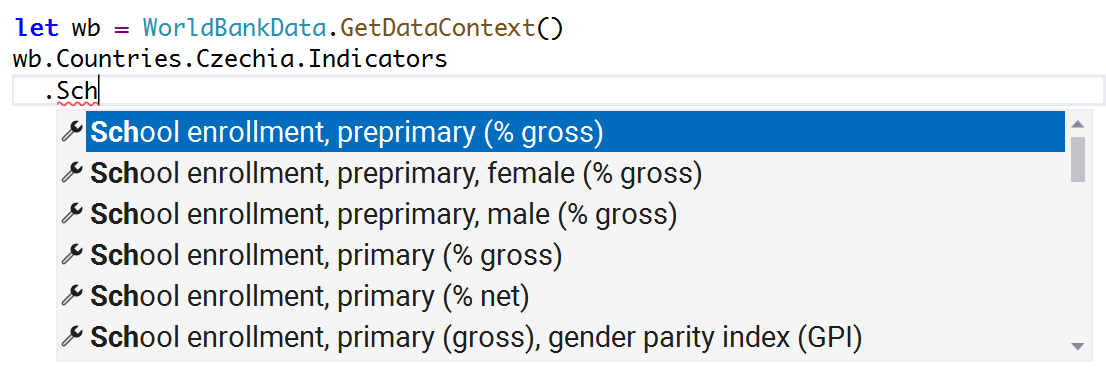
\includegraphics[width=0.7\textwidth]{fig/worldbank.png}
  \caption{F\# code editor showing completions offered by the World Bank type provider.}
  \label{fig:worldbank}
\end{figure}

\section{Motivation}
\label{sec:motivation}

Computer scientists studying programming have long focused on programming languages as syntactic
entities, sometimes neglecting the interactive environments in which they are inevitably
embedded \cite{rpg-2012-revolution}. Notably, in many of the motivating examples that we draw
from in this section, the interactive aspect of the system is only described in supplementary
materials \cite{brady-2015-idris,syme-2013-inforich,altenkirch-1994-alf}. Only recently, programming
language theory started to be used to study interactive environments
\cite{adams-2025-grove,mayer-2018-bidirectional}. Our work contributes to this research direction.

The following sections review four different instances of the choose-your-own-adventure
interaction pattern. In all of those, an interactive editor offers the user some kind of~a~com\-pletion list during working with the system.

\subparagraph{Type providers.}

F\# type providers \cite{syme-2013-inforich} are a mechanism for integrating external data
sources into the F\# type system. A type provider is a compiler extension, loaded and
executed at compile-time and at edit-time. It can run arbitrary code to read the structure of
external data and use it to generate a suitable statically-typed representation of the
data, typically as objects with members. Type providers can, for example, infer the type from a
sample JSON \cite{petricek-2016-fsdata} or read a database schema.

The example in Figure~\ref{fig:worldbank} shows a simple type provider for accessing information
from the World Development Indicators database. The provided \ident{wb} object allows the programmer
to access any indicator of any country in the database by choosing an appropriate \ident{[Country]}
and an \ident{[Indicator]} in a chain of members
\ident{wb}.\ident{Countries}.\ident{[Country]}.\ident{Indicator}.\ident{[Indicator]}.
The result is a time series with values for the given indicator and a country. More generally,
the example can be seen as a special case of a type provider for slicing n-dimensional
data cube \cite{petricek-2022-thegamma} -- we choose a fixed value for two of the three
dimensions (country, indicator, time).

When using the type provider, the user types the first line of code and triggers auto-completion
by typing \ident{wb} followed by the dot. The rest of the code is constructed by choosing an
option from a list and typing another dot.\footnote{This interaction pattern has been
lightheartedly called \emph{dot-driven development} by Phil Trelford \cite{seemann-2021-head}.}


\newpage

\begin{figure}[t]
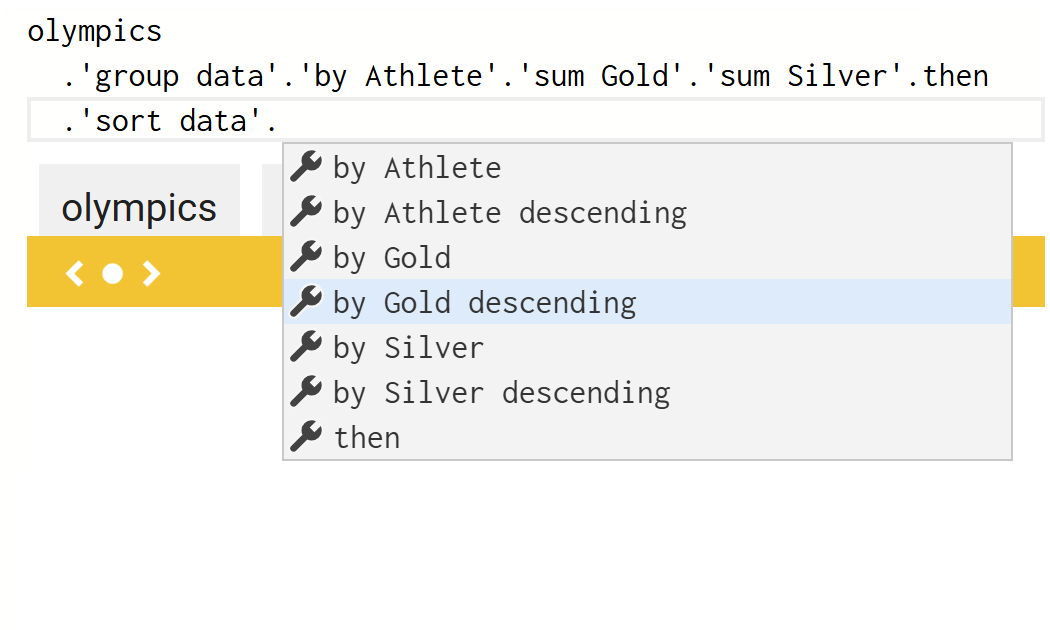
\includegraphics[width=0.48\textwidth]{fig/thegamma1.png}~~
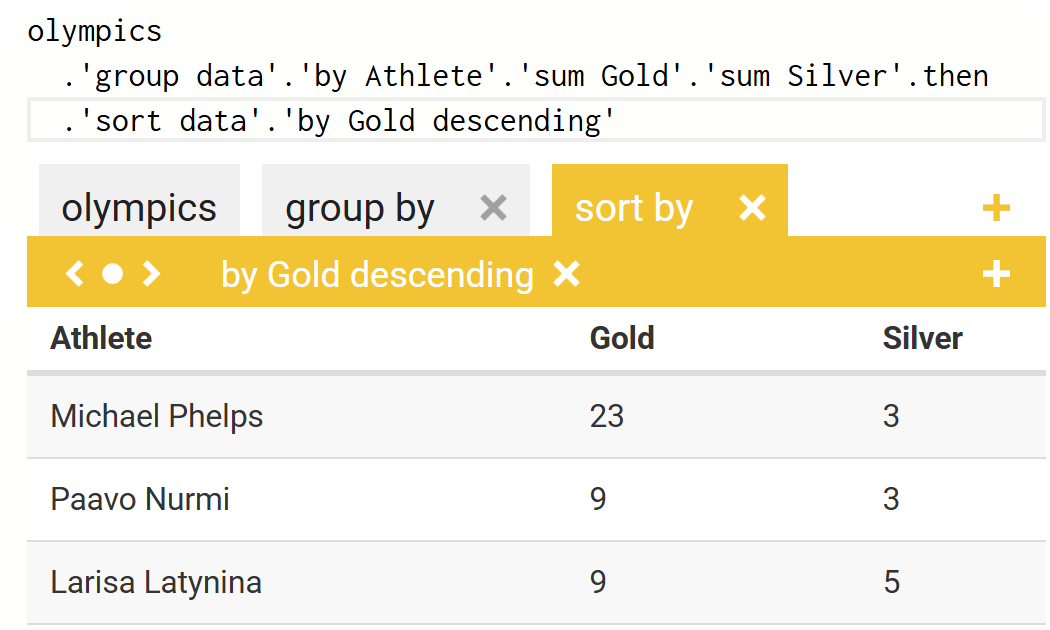
\includegraphics[width=0.48\textwidth]{fig/thegamma2.png}
\caption{Constructing a query in The Gamma. We count the number of gold and silver medals for
each athlete and sort the data by the number of gold medals.}
\label{fig:thegamma}
\end{figure}

\subparagraph{Data exploration.}

The Gamma~\cite{petricek-2022-thegamma} is a programmatic data exploration environment
for non-programmers. In The Gamma, type providers are the primary programming mechanism. They
are used not just for data access, but also for constructing queries.

The type provider shown in Figure~\ref{fig:thegamma} lets the user construct an SQL-like query by
repeatedly choosing operations and their parameters \cite{petricek-2017-dotdriven}. It keeps track
of the schema and uses it to generate all possible valid parameters. When sortin data, it generates
an object with two members for each columns -- one for ascending and one for descending sort.
Similarly, the grouping operation first offers all columns as possible grouping keys and then
lets the user choose from a range of pre-defined aggregations (sum, count, average, concatenate).
The system also evaluates the query on the fly, providing a live preview during editing \cite{petricek-2020-live}.

The interaction pattern is the same as before. After the usertriggers auto-completion, they
repeatedly select an operation and its parameters to construct a query. One notable difference
is that the structure of the generated types is potentially infinite (the user can keep adding
further operations) and so the types are generated lazily.

\subparagraph{AI assistants.}

The third instance of the choose-your-own-adventure interaction pattern comes from the work on
semi-automatic data wrangling tools known as AI assistants \cite{petricek-2023-aias}.
An AI assistant guides the analyst through a data wrangling problem such as reconciling mismatched
datasets, filling missing values or inferring data format and types. An AI assistant solves
the problem automatically and suggests an initial data transformation, but it also generates a
number of constraints that the user can choose from to refine the initial solution. If the initial
solution is not correct, the user chooses a constraint and the AI assistant runs again, suggesting
a new data transformation that respects the constraint.

Figure~\ref{fig:aia} shows an example. It uses the datadiff \cite{sutton-2018-datadiff} AI
assistant, running in a Wrattler notebook \cite{petricek-2018-wrattler}, to merge broadband
quality data published by Ofcom for two subsequent years. The format of the CSV files for the
two years differs. Columns were added, removed, renamed and their order has changed. In the
example, we selected 6 columns from the year 2015 and want to find matching data from 2014.

When the AI assistants runs automatically, it correctly maps the numerical columns, but it
incorrectly maps the \ident{Urban.rural} (2014) column to \ident{Nation} (2015). This happens
because both columns are categorical and have three values with similar distribution. A data
analyst can easily spot the mistake. They click the ``+'' button to add a constraint and choose
\ident{Don't match `Urban.rural' and `Nation'} to specify that the two columns should not be matched.
Datadiff then runs again and finds the correct matching.

\begin{figure}[t]
  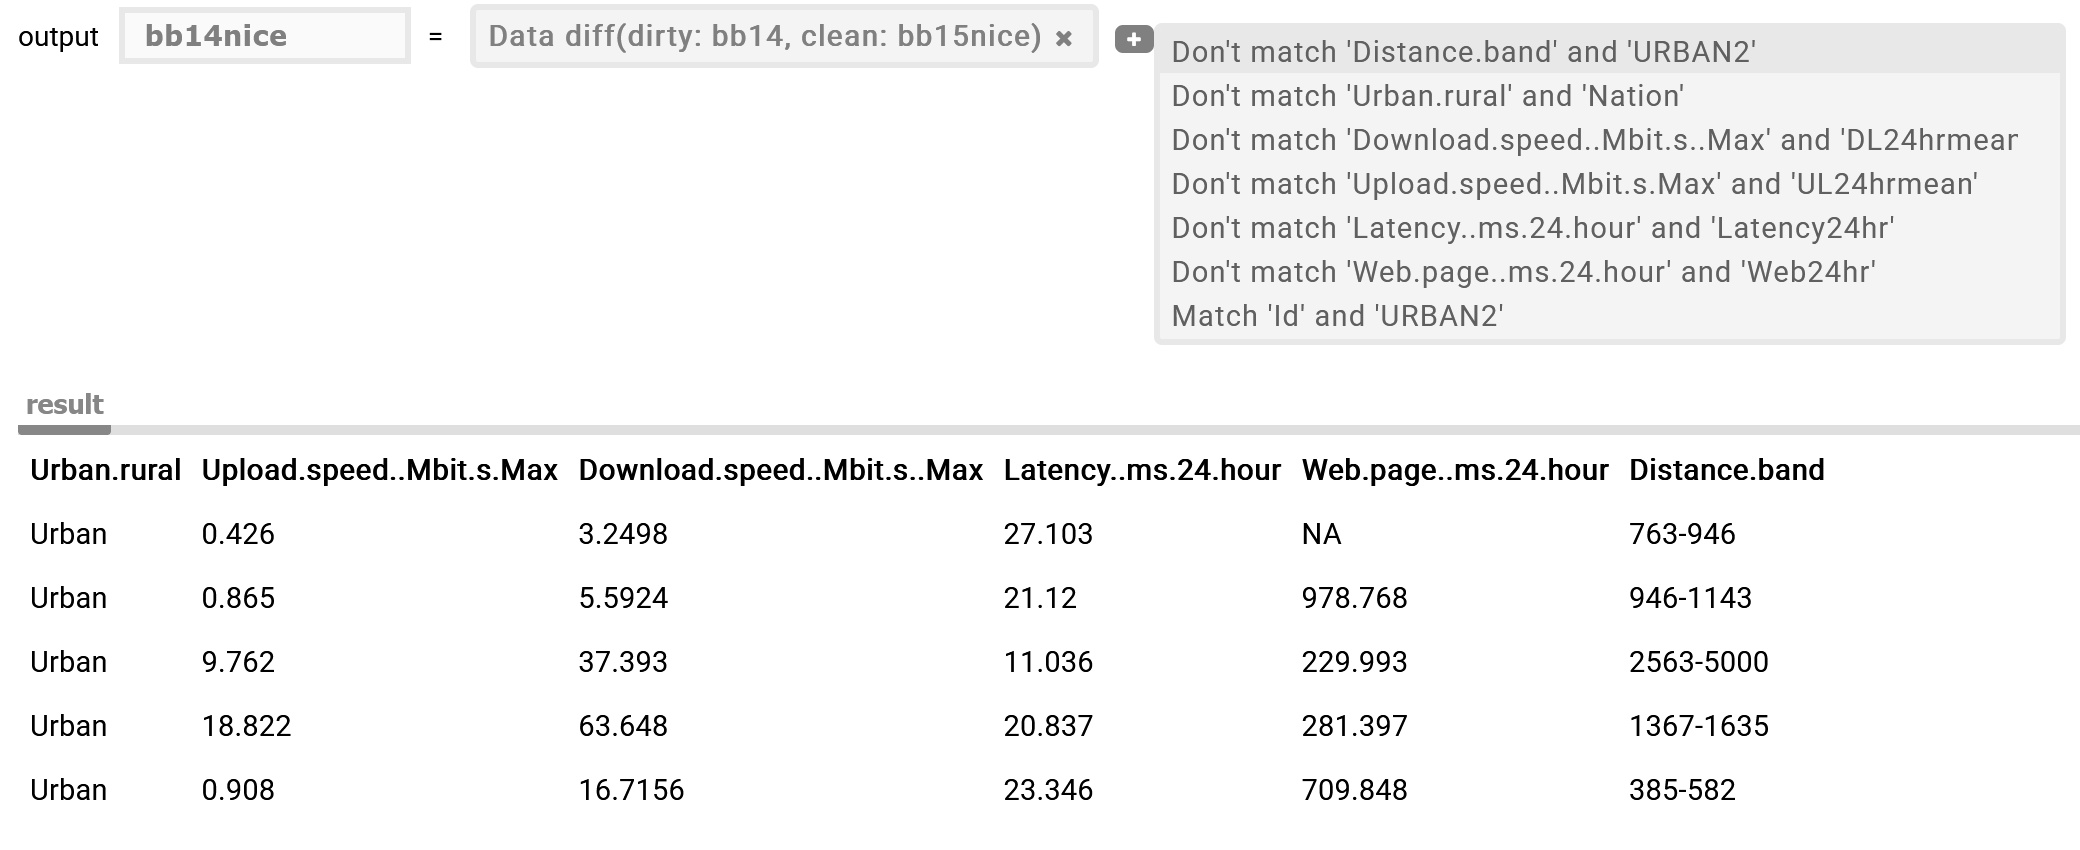
\includegraphics[width=0.9\textwidth]{fig/aia.png}
  \caption{Using the datadiff AI assistant to reconcile the structure of the two datasets.
    The user is offered a list of constraints to prevent or force matching between specific columns.}
  \label{fig:aia}
\end{figure}

~

The interaction patter is the same as in the previous two cases. The analyst constructs the
correct data transformation by repeatedly choosing from a list of options, until they obtain
the desired result. However, the way the interaction pattern is implemented differs.
First, in the case of type providers, we are gradually constructing a program by adding operations to
a method chain. Now, the AI assistant synthesizes a data transformation (program) and we are
gradually adding constraints to control the synthesis. Second, in the case of type providers,
the completion list offered all possible members of the object. Now, the list offers
constraints recommended by the AI assistant which may not be complete.

\newpage

\begin{figure}[t]
  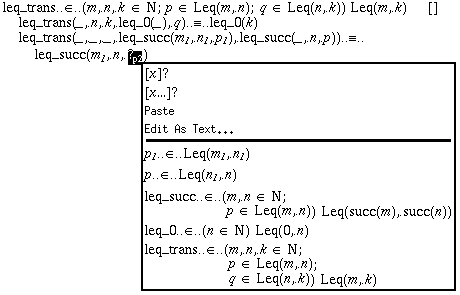
\includegraphics[width=0.6\textwidth]{fig/alf.png}
  \caption{Constructing a proof of the transitivity of the $\leq$ relation in the \textsc{Alf}
    editor. The user is offered a range of variables and constructors in scope at the current
    location. \cite{altenkirch-1994-alf}}
  \label{fig:alf}
\end{figure}

\subparagraph{Interactive theorem provers.}
A fourth example of the choose-your-own-adventure interactive pattern can be found in interactive
theorem provers. When writing programs in systems like Idris \cite{brady-2021-idris2}, the
user typically works by stating the desired conclusion and filling the implementation with a hole.
The system provides a range of interactive editing capabilities to fill the holes \cite{mcbride-1999-dependently}.
It can, for example, generate a case split or search for a proof \cite{brady-2015-idris}.

Systems like Idris provide key bindings to invoke the completions, but the functionality could
also be offered through a user interface. An example that illustrates this is the interactive editor
for the \textsc{Alf} theorem prover \cite{magnusson-1994-alf}, which is based on the refinement of
an incomplete proof object \cite{altenkirch-1994-alf}. This is illustrated in Figure~\ref{fig:alf}.
The user is proving the transitivity of the $\leq$ relation for Peano arithmetic natural numbers.
They pattern match on the proof argument $p$ and complete the first branch. For the second branch,
they need to fill a hole $?_{p2}$ (called a wildcard in \textsc{Alf}). They trigger a completion
and a pop-up menu shows the available variables and constructors, including \ident{leq\_trans} that
can be used to complete the proof. After choosing \ident{leq\_trans}, two new holes are generated
for its arguments. Those can be, again, filled interactively, by choosing $p_1$ and $p$ from the
completion.

The interaction pattern is again the same. The user repeatedly triggers a completion and uses
it to refine and complete their proof by filling holes. There are subtle differences too. Unlike
with AI assistants, each completion directly refines the proof that the user is editing. Unlike
with type providers, a completion may generate multiple new holes, rather than just adding to a
chain of operations.

The \textsc{Alf} editor is a historical example, but a similar user interface could be built for
systems like Idris or Coq. The two would work differently. As in \textsc{Alf}, Idris source code
represents the proof itself and a completion would replace a hole with a suggested term. In Coq,
the proof is a series of tactic invocations and so selected completions would be added to this
list and would form a trace of the interaction with the user.

\newpage

\begin{figure}[t]
  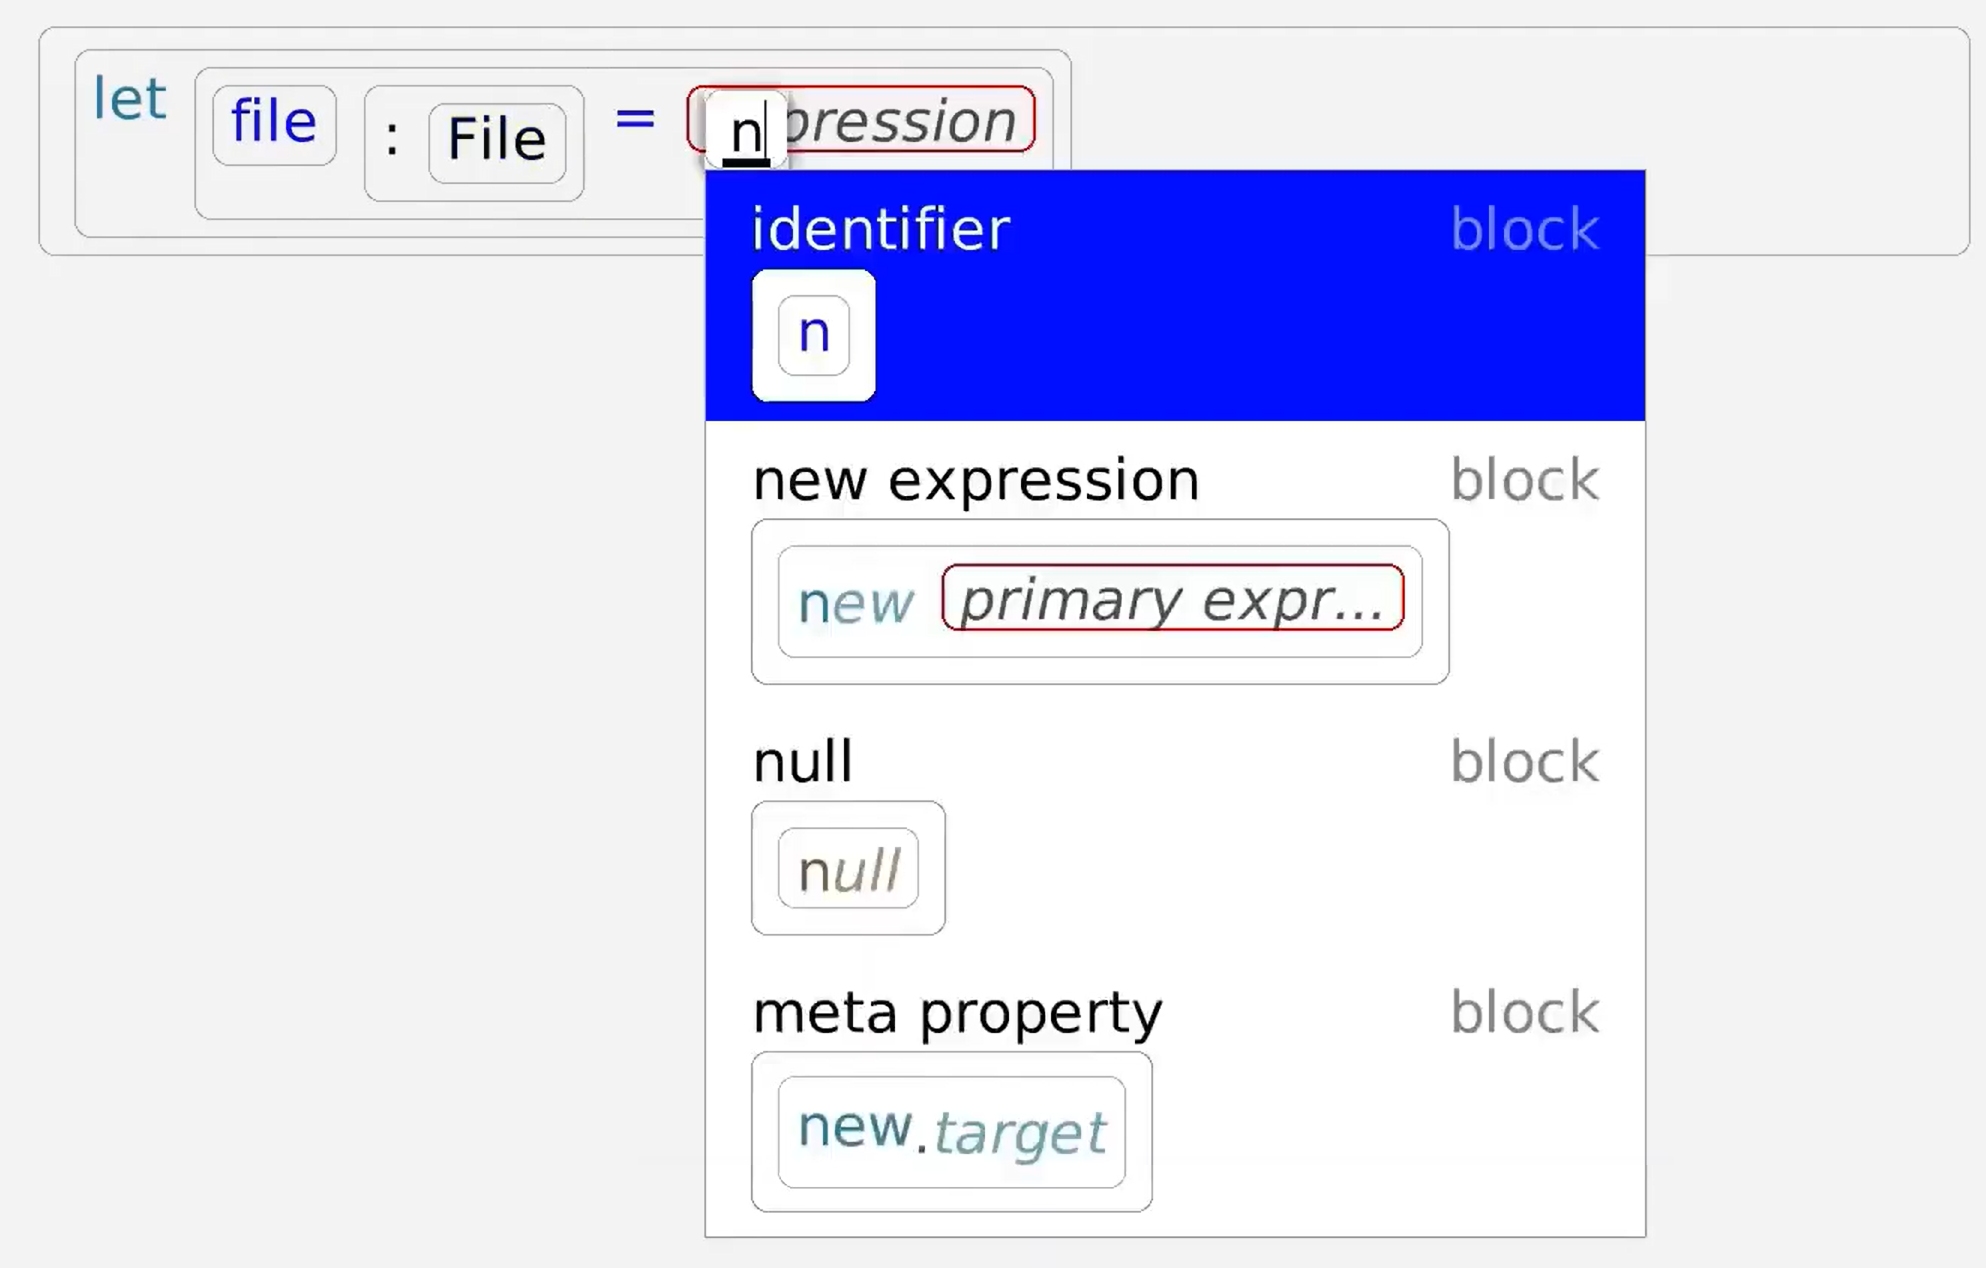
\includegraphics[width=0.55\textwidth]{fig/sandblocks.png}
  \caption{Constructing a program using the Sandblocks structure editor \cite{beckmann-2023-all}.
    The user is typing the start of an expression and context menu offers possible production
    rules according to a grammar.}
  \label{fig:sand}
\end{figure}

\subparagraph{Structure editors.}
Structure editors make it possible to construct programs by manipulating the abstract syntax tree
of a program rather than by working with textual representation. The interaction with a structure
editor can be based on menus \cite{teitelbaum-1981-synth}, key bindings \cite{weber-2017-editors},
tiles~\cite{moon-2022-tylr} and a range of other approaches.

Sandblocks~\cite{beckmann-2023-all} is an example of a recent structure editor that is interesting
for multiple reasons. First, the editor is automatically generated from a grammar. Second, the
editor combines keyboard input with context menus (Figure~\ref{fig:sand}). In the above example,
the user is typing code and needs to fill a placeholder for an expression. After they type the
start of the expression, the editor offers a completion list with possible production rules from
the grammar that are valid in the given context and are compatible with the text typed so far. The
user can continue typing (to further refine the recommendation), but they can also select a rule
from the menu. This completes the expression according to the production rule, leaving further
empty holes in the code.

In Sandblocks, the context menus serve more as hints and users of the editor often
construct programs through typing, but the system illustrates the fact that structure editors
can also be based on the interaction pattern captured in this paper. The editor can offer
all possible production rules based on the given grammar and the user could construct an
entire program by choosing one of the rules (and manually entering primitive terminals such as
strings and identifiers).

\newpage

\section{Formal model}
\label{sec:calculus}

A system that implements the choose-your-own-adventure interaction pattern repeatedly offers
the user a range of options to choose from. Each of the options is designated by an identifier.
The system also maintains a state during the process which determines subsequent options. The state
may not be visible to the user, but the user can always explicitly request the program constructed
so far.

We can think of the interaction with the system as navigating through a tree structure, starting
from a root and choosing one of the possible branches in each step.\footnote{Serving as another
evidence for the surprising effectiveness of the concept of a tree \cite{nesetril-2005-strom}.}
In the following definition, the key $\choices$ operation can thus be seen as returning
branches of a given node.

\begin{definition}[Choose-your-own-adventure system]\label{def:calculus}
Given expressions $e\in \mathbb{E}$ and states $\sigma \in \Sigma$, a choose-your-own-adventure
system is a pair of operations \choices, \select\ such that:

\vspace{-0.5em}
\raggedright
\begin{itemize}
  \item $\choices(\sigma) = \{\iota_1\mapsto\sigma_1, \ldots, \iota_n\mapsto\sigma_n\}$ is
    an operation that takes a state and \\ generates options designated by an identifier $\iota_i$
    and represented by a state $\sigma_i$,
  \item $\select(\sigma) = e$ is an operation that returns generated program for a given state.
\end{itemize}
\end{definition}

The definition is not a programming language calculus in the usual sense in that it does not
define a concrete syntax with reduction rules. It is an abstract algebraic structure that captures
the structure of a system that supports the choose-your-own-adventure interaction pattern.
The definition is close to that of an AI assistant \cite{petricek-2023-aias}, which is written
using a language specific for the data wrangling domain (such as cleaning scripts or input and
output data) but is structurally similar. It is also worth noting that the definition may describe
not just trees, but also graphs with cycles -- a system can return to a previously visited state.
This is not practically useful, but it does not pose a theoretical problem.

\subparagraph{Expression completion.}
One of the subtle questions about the choose-your-own-adventure pattern raised in the introduction
is whether a trace of the interaction can be reconstructed from the source code of an interactively
constructed program. That is, if we follow a sequence of choices $\iota_1, \ldots, \iota_n$ to
construct a program $e$, is it possible to recover the original sequene of choices from the
program $e$.

The choose-your-own-adventure interaction pattern is typically used to complete a partial program.
To model this, we assume that the host language has a notion of a hole, written as~$?$
and that a user can select a part of program to invoke the completion on. When invoked on
an expression containing multiple holes, the system can start by completing the first hole.

We write $E[e]$ for a completion context, akin to evaluation contexts in operational semantics.
We assume that, for a program containing a hole in a completion context $E[?]$, we can construct
an initial choose-your-own-adventure state using an operation $\ident{init}(E[?])=\sigmaN$.

\begin{definition}[Expression completion]
An expression $E[?]$ is completed as $E[e]$ through an interaction with
a choose-your-own-adventure system consisting of \choices\ and \select\ if:

\vspace{-0.5em}
\raggedright
\begin{enumerate}
\item $\ident{init}(E[?]) = \sigmaN$ obtains the initial state of a choose-your-own-interaction system,
\item $\sigma_n$ is a system state such that $\forall i\!\in\! 1\ldots n\;.\;(\iota_i\mapsto\sigma_i)\in\choices{(\sigma_{n-1})}$,
  i.e.,~the user\\ makes a series of choices resulting in a final state of the system $\sigma_n$,
\item $E[e]$ where $e=\select(\sigma_n)$, i.e.,~the final program is constructed by replacing the hole
  in the completion context with the expression $e$ generated from $\sigma_n$.
\end{enumerate}
\end{definition}

As we will see when we revisit the earlier examples formally, this way of invoking a choose-your-own-adventure
system is used, for example, in the case of interactive theorem provers like \textsc{Alf} or Idris.
In those systems, the user triggers the completion on a proof (program) containing a hole.
They then fill the hole and, possibly iteratively, further holes in the generated proof. The final
expression is embedded in the source code, but it does not indicate what options, identified by
$\iota_1, \ldots, \iota_n$, were selected in the process.

\subparagraph{Reconstructible completion.}
In many choose-your-own-adventure systems, it is possible to reconstruct a trace of the interaction
through which a program was constructed. This is the case with type providers, where a user chooses
a sequence of object members to be accessed and those members directly appear in the source code.
The same would be the case in a completion system for Coq that would offer tactics to apply,
becuase the resulting proof would contain a record of the selected tactics.

For systems such as type providers, we say that that expression completion is \emph{reconstructible}.
To capture the notion formally, we again need the \ident{init} operation, but also an operation
\ident{decode} that extracts identifiers of invoked completions from an expression:

\begin{definition}[Reconstructible expression completion]
An expression $E[?]$ is reconstructibly completed as $E[e]$ through an interaction with
a choose-your-own-adventure system consisting of \choices\ and \select\ if:

\vspace{-0.5em}
\raggedright
\begin{enumerate}
\item $E[?]$ is completed as $E[e]$ using \ident{init}, \choices\ and \select\\
  through a series of choices designated by identifiers $\iota_1, \ldots, \iota_n$,
\item it also holds that $\ident{decode}(e)=(\iota_1, \ldots, \iota_n)$.
\end{enumerate}
\end{definition}

If the integration of a choose-your-own-adventure system with a host programming language
uses reconstructible expression completion, we can recover the choices through which the user completed
an expression $e$ in a completion context $E[e]$, assuming they used the interactive system rather
than entering the code directly. This also means that we can reconstruct the final state $\sigma_n$
of the system by starting from $\ident{init}(E[?])$ and following the choices specified by
$\iota_1, \ldots, \iota_n$.

\newpage
\section{Examples}
\label{sec:examples}

We now revisit the four examples from Section~\ref{sec:motivation} and show how they fit the
above formal model. All four examples rely on some domain-specific logic. We describe what
information the logic provides, but do not model it formally. This has been done elsewhere,
in works describing the individual systems.

To show how the model lets us distinguish subtle details of interactive programming systems,
we start with a model of data exploration system that is inspired by The Gamma, but differs in
one notable way. We then discuss type providers more generally and show how to correctly model
The Gamma. We then revisit the remaining two examples.

\subsection{Data exploration}
\label{sec:examples-data}

In The Gamma, the choose-your-own-adventure interaction pattern is used to construct a
query that transforms the given input data. The query is a sequence of operations with parameters,
$\op(p_1, \ldots, p_n)$, loosely modelled after relational algebra \cite{codd-1970-relational}.

In The Gamma, the query is hidden from the data analyst. Behind the scenes, the system generates
objects with members and the identifiers designating individual options are the names of those
members. The operation is encapsulated in the code of the accessor of the member. In the
simplified model in this section we ignore this fact. The model presented here directly
generates code that calls the underlying operations. For example, assume that the user makes
the following choices:
\[
\textnormal{\ddident{group data}\,.\,\ddident{by Athlete}\,.\,\ddident{sum Gold}\,.\,\ddident{count all}\,.\,\ddident{then}}
\]
In The Gamma, the individual identifiers become object members and they are included as
a member chain in the generated code. In the following simplified model, the completion
instead fills the hole with an expression representing the operation:
\[
\ident{group}(\texttt{"Athlete"}, \ident{sum}(\texttt{"Gold"}), \ident{count}())
\]
The two approaches have different human-computer interaction trade-offs. In terms of cognitive
dimensions \cite{green-1989-cogdims,blackwell-2003-cogdims}, the latter has a greater closeness
of mapping, while the former is less cognitively demanding to read for a non-programmer.
As discussed in Section~\ref{sec:properties}, the two implementations of the choose-your-own-adventure
interaction pattern also differ in terms of their formal properties.

\subparagraph{Formal model.}
The options generated by The Gamma let the user select both the next operation and the parameters
of the previously selected operation. The available operations and parameters are generated
based on a schema $S$ that is transformed by the operations. The state of the system $\sigma$
contains the current schema $S$ and the operations applied so far. In the following, we write
$\op(\boldsymbol{p})$ for an operation with a vector of parameters:
\[
\sigma = S, \vect{\op_1(\boldsymbol{p_1}), \ldots, \op_n(\boldsymbol{p_n})}\\
\]
The behaviour of the $\choices$ operation depends on whether the last operation in the sequence
expects further parameters or whether it is fully-specified. In the first case, the recommendation
engine generates possible additional parameter values $p', p'', \ldots$ based on the schema $S$,
the operation $\op_n$ and the already known parameters $\boldsymbol{p_n}$.
The $\choices$ operation then generates options that add the additional parameter. We generated the
identifiers $\iota',\iota'',\ldots$ based on the state and the parameter value, such as
\ddident{by Gold descending}. Note that adding a parameter may also result in a new schema
$S', S'', \ldots$ (which the recommendation engine computes based on the previous schema and the new parameter):
\[
\begin{array}{l}
\choices(S, \vect{\op_1(\boldsymbol{p_1}), \ldots, \op_n(\boldsymbol{p_n})}) =\\
\qquad \{\; \iota' \mapsto (S', \vect{\op_1(\boldsymbol{p_1}), \ldots, \op_n(\boldsymbol{p_n},p')}), \\
\qquad\;\;    \iota'' \mapsto (S'', \vect{\op_1(\boldsymbol{p_1}), \ldots, \op_n(\boldsymbol{p_n},p'')}), ~\ldots~\}
\end{array}
\]
If the last operation takes no further parameters, the system produces a choice
of possible next operations $\op', \op'', \ldots$. Again, we are also given new schemas $S', S'', \ldots$
and we generate identifiers $\iota',\iota'',\ldots$ based on the operation name. The $\ident{choices}$
operation then returns options that add the additional operation:
\[
\begin{array}{l}
\choices(S, (\op_1(\boldsymbol{p_1}), \ldots, \op_n(\boldsymbol{p_n}))) =\\
\qquad \{\; \iota' \mapsto (S', \vect{\op_1(\boldsymbol{p_1}), \ldots, \op_n(\boldsymbol{p_n}), \op'()}), \\
\qquad \;\; \iota'' \mapsto (S'', \vect{\op_1(\boldsymbol{p_1}), \ldots, \op_n(\boldsymbol{p_n}), \op''()}), ~\ldots~\}
\end{array}
\]
Finally, the $\select$ operation takes the state $\sigma$ and generates an expression that represents
the data transformation. This is only possible if all parameters are fully-specified. For simplicity,
assume that $k$ is the index of the last fully-specified operation (either $n$ or $n-1$). If the
host language lets us compose functions using $f\circ g$, we can write:
\[
\select(S, (\op_1(\boldsymbol{p_1}), \ldots, \op_n(\boldsymbol{p_n}))) = \op_1(\boldsymbol{p_1}) \circ \ldots \circ \op_k(\boldsymbol{p_k})
\]
The recommendation engine behind The Gamma provides a domain-specific logic for generating
possible operations and their parameters based on the current schema of the data. As the above
definition shows, this underlying engine can be easily exposed through the common
choose-your-own-adventure interface.

\subsection{Type providers}
\label{sec:examples-tps}

The type provider mechanism in F\# operates at the level of the type system. It is not a merely an
editor feature. A type provider for a data source, such as the World Development Indicators database,
generates a collection of types that model the external data source. In F\#, the types are classes
with members that implement the logic to retrieve data at runtime.

The auto-completion mechanism in F\# code editors, which implements the choose-your-own-adventure
interaction pattern, is not specific to type providers. It offers a list of members of an object
based on its type. We model the completion as an iterative process, repeatedly adding further
members to a chain. The state $\sigma$ thus consists of an initial expression on which the
completion is invoked, a chain of selected members and the type of the last member.

To model the completion mechanism, we also need to model information about types. We loosely
follow the Foo calculus model \cite{petricek-2016-fsdata} and write $\mathbb{C}$ for a set
of class definitions, each consisting of an implicit class constructor and a collection of
members $M$:
\[
\begin{array}{rcl}
\sigma &=& e . \iota_1 . \lbrack\ldots\rbrack . \iota_n, C\\
\mathbb{C} &=& \{ C \mapsto \ident{type}~C(\overline{x:\tau}) = \overline{M},~\ldots~ \}\\
M &=& \ident{member}~\iota\!:\!C=e
\end{array}
\]
Each member in the Foo calculus consists of a of a name $\iota$, return type $C$ and implementation
$e$. For our purposes, we only need the type information and so the operations that define the
choose-your-own-adventure are parameterized by the set of classes $\mathbb{C}$.

The $\choices_\mathbb{C}$ operation finds the class definition corresponding to the type of the
last member in the current chain. It offers choices appending each of the available
members to the current chain. The $\select_\mathbb{C}$ operation returns the constructed
member chain:

\[
\begin{array}{l}
\choices_\mathbb{C}(e . \iota_1 . \lbrack\ldots\rbrack . \iota_n, C) =\\
\qquad \{\; \iota' \mapsto (e . \iota_1 . \lbrack\ldots\rbrack . \iota_n . \iota', C')\\
\qquad \;\; \iota'' \mapsto (e . \iota_1 . \lbrack\ldots\rbrack . \iota_n . \iota'', C''), ~\ldots~\}\\[1em]
\end{array}
\]\vspace{-2em}
\[
\begin{array}{rcl}
\quad \textnormal{where}~\mathbb{C}(C) &=& \ident{type}~C(\overline{x:\tau}) = M', M'', \ldots\\
\quad \textnormal{and}~M' &=& \ident{member}~\iota'\!:\!C'=e'
\end{array}
\]\vspace{-0.5em}
\[
\select_\mathbb{C}(e . \iota_1 . \lbrack\ldots\rbrack . \iota_n, C) = e . \iota_1 . \lbrack\ldots\rbrack . \iota_n
\]
The model does not directly refer to type providers. Those are responsible solely for generating
the type definitions in $\mathbb{C}$ as documented in earlier work \cite{petricek-2016-fsdata}.
It is worth noting that the type provider for data exploration, implemented by The Gamma,
additionally needs to generate classes lazily \cite{petricek-2017-dotdriven}. To model this aspect,
the simple lookup $\mathbb{C}(C)$ needs to be replaced with an operation that returns the type
definition, alongside with a new context $\mathbb{C}'$ that contains additional generated
type definitions (return types for all the members of the class~$C$).

The model follows the internal mode of embedding the interaction in the program. It is easy to
define the \ident{decode} operation that takes the resulting generated expression and returns the
sequence of choices, because the choices are items of the member chain. A slight caveat is that
the completion is not invoked on an empty hole, but on a hole that contains the initial expression
on which the completion is applied. We can model this using filled holes \cite{omar-2019-holes}
and write $?_e$ for a hole containing the initial expression $e$. The $\ident{init}(?_e)$ operation
then returns $e$ alongside with an empty chain and the type of $e$.

As noted earlier, The Gamma does not embed query expressions directly into the generated code.
It uses the same model as type providers and generates choices as members of
types behind the scenes. We return to the differences between the two models in
Section~\ref{sec:properties}.

\subsection{AI assistants}
\label{sec:examples-aias}

AI assistants guide the analyst through a data wrangling task. They
generate a data cleaning script, taking into account constraints selected by the user.
Most AI assistants obtain the script by performing statistical optimization with respect
to a set of constraints specified by the user. That is, they look for an expression from the
set of all possible expressions that optimizes some objective function that assigns score to
the expression with respect to the given input data. Note that AI assistants do not iterate
over all possible expressions. They use a machine learning method to approximate a solution
to the problem.

An optimization-based AI assistant \cite{petricek-2023-aias} thus provides another, very
different, way of implementing the choose-your-own-adventure pattern. The assistant operates
with respect to some input data $X$ that does not change during the interaction and so we
parameterize the choose-your-own-adventure calculus operations by the data.
The input data $X$ can be actual input data or a representative sample and so the AI assistant
can be use past data to infer a cleaning script that will be used on new inputs.

The state $\sigma$ consists of a set of constraints specified by the user. We write
$c$ for individual constraints and $\boldsymbol{c}$ for a set of constraints. The initial
state is an empty set:
\[
\begin{array}{rcl}
\sigma &=& \{ c_1, \ldots, c_n \}\\
\sigmaN &=& \emptyset
\end{array}
\]
Unlike in the previous examples, the crucial logic of an AI assistants is implemented in the
$\select$ operation. The operation runs the optimization algorithm to choose the best cleaning
script for given constraints. Formally, this can be written using the $\argmax$ operator which
finds an argument (an expression) for which the given function (scoring function) is maximized.
The user-specified constraints can either restrict the set of possible expressions or influence
the scoring function. More formally, we assume that:

\begin{itemize}
\item $E_{\boldsymbol{c}}\subseteq E$ is a set of expressions that respect constraints $\boldsymbol{c}$,
\item $Q_{\boldsymbol{c}}(X, e)$ is a scoring function with respect to the constraints $\boldsymbol{c}$,
  which returns the score of an expression $e$, i.e., how good $e$ is at cleaning the data $X$.
\end{itemize}

\noindent
For a given set of constraints $\boldsymbol{c}$, the $\select$ operation looks
for $e\in E_{\boldsymbol{c}}$ with the largest score:
\[
\select_X(\boldsymbol{c}) = \argmax_{e \in E_{\boldsymbol{c}}} Q_{\boldsymbol{c}}(X, e)
\]
The actual implementation of the optimization uses various machine learning techniques to
find the optimal expression. In case of datadiff, $X$ is a pair of datasets $X_1, X_2$ to be
reconciled. The AI assistant uses the Hungarian algorithm \cite{sutton-2018-datadiff} to construct
a matching of columns from $X_1$ and $X_2$. The generated expression is a sequence of patches
that can be applied to $X_2$ in order to reconcile its structure with the sturcture of $X_1$.
The constraints specified by the user restrict the space of possible column matchings and so they
affect $E_{\boldsymbol{c}}$. The scoring function $Q_{\boldsymbol{c}}$ is independent of
the constraints and computes a sum of distances between the statistical distributions of the
columns from $X_1$ and a patched version of $X_2$.

The $\choices$ operation is responsible for generating possible constraints that the user may
want to add to guide the inference. AI assistants typically offer the user options to prevent
or adapt some aspect of the cleaning logic inferred by the system. For example, if datadiff
matches two columns, it will offer a constraint to prevent the matching. It also generates
constraints that let the user force a specific matching.

To implement $\choices_X$, optimization-based AI assistants first call $\select_X(\sigma)$ to
get the best expression $e$. Based on this, they generate possible constraints $c_1, c_2, \ldots$
that the user may want to choose from. The identifiers $\iota_1,\iota_2, \ldots$ provide a
human-readable description of the constraints. Note that this operation is specific to the particular
AI assistant. The $\choices_X$ operation then offers a list of constraint sets where the additional
constraint is added to the previously collected set:
\[
\choices_X(\boldsymbol{c}) = \{\iota_1 \mapsto \boldsymbol{c}\cup\{ c_1 \}, \iota_2\mapsto\boldsymbol{c}\cup\{ c_2 \}, \ldots\}
\]
The integration of an AI assistant, as described here, has to follow the external mode of embedding.
The interaction with the assistant results in a cleaning script (expression), but there is no way
of reconstructing the constrains used to guide the optimization. To support internal embedding, the
$\select$ operation would need to explicitly include the constraints in the resulting expression.
However, rerunning the $\select$ operation with the same constraints may result in a different
cleaning script if the machine learning algorithm is probabilistic.

\newpage

\subsection{Theorem proving}
\label{sec:examples-thm}

In the previous three sections, we showed how existing formally well-documented systems fit the
choose-your-own-adventure interaction pattern. Although interactive theorem provers and editors
for dependently typed languages implement similar kinds of interactions, there is no well-documented
system that exactly fits the pattern. The closest example is perhaps the recently envisioned
mixed-mode interaction theorem prover \cite{verter-2024-mixed}. Rather than reframing the
implementation of an existing system, this section thus outlines a possible implementation.

\subparagraph{Theorem provers.}
There are two approaches to interacting with an interactive theorem prover. In Coq, the user
writes a sequence of tactics that transform proof goals. In Agda or Idris, the user writes a
term, or program, of a type that represents the theorem. Interactive editors exist for both
types of systems. For Coq, the \texttt{Company-Coq} \cite{pitclaudel-2016-companycoq,aspinall-2000-general}
extension offers auto-completion, which recommends available tactics, hypotheses and local
definitions, but it does not filter them based on what is valid in a given context.
For Idris, the interactive editor \cite{brady-2015-idris} offers a range of commands that
transform the selected term by adding a case split, a missing case or by automatically searching
for a proof. In Idris, the system produces valid completions, but those cover only a small number
of situations.

Despite the different ways of working, an implementation of the choose-your-own-adventure
pattern for both types of systems would be similar. Based on the sub-goal that the user is
currently proving, the system would recommend a range of tactics that can be applied to the
sub-goal. In the case of Coq, the selected tactic would be added to the sequence. In Idris, the
selected tactic would be applied to transform the current term. The difference is in the mode of
embedding. A system for Coq would provide internal embedding in that the selected option is added
to the proof source code. (Much like selecting a completion when using type providers appends a
member access.) A system for Idris-like language would use the tactic to transform the term,
making it impossible to reconstruct the sequence of applied tactics as in the external mode of
embedding.

\begin{figure}
\[
\begin{array}{lcl}
\boxed{\Gamma \vdash \tau \Rightarrow e}\\[1em]
\dfrac{}{\Gamma,x:\tau \vdash \tau \Rightarrow x}~\ident{(syn-var)} &\quad&
\dfrac{}{\Gamma \vdash \tau \Rightarrow ?_\tau}~\ident{(syn-hole)}\\[2em]
\dfrac{\Gamma,x:\tau_1\vdash \tau_2 \Rightarrow e}{\Gamma \vdash \tau_1 \rightarrow \tau_2 \Rightarrow \lambda x.e}~\ident{(syn-lambda)}&&
\dfrac{\Gamma \vdash \tau_1\rightarrow\tau_2 \Rightarrow e_1 \quad \Gamma \vdash \tau_1 \Rightarrow e_2}{\Gamma \vdash \tau_2 \Rightarrow e_1~e_2}~\ident{(syn-app)}\\[2em]
\dfrac{b\in \{\ident{true},\ident{false}\} }{\Gamma \vdash \ident{bool} \Rightarrow b}~\ident{(syn-bool)} &\quad&
\dfrac{\Gamma \vdash \tau \Rightarrow e_1 \quad \Gamma \vdash \tau \Rightarrow e_2 \quad \Gamma \vdash \ident{bool} \Rightarrow e}{\Gamma \vdash \tau \Rightarrow \ident{if}~e~\ident{then}~e_1~\ident{else}~e_2}~\ident{(syn-cond)}\\
\end{array}
\]
\caption{Illustrative set of simple type-directed program synthesis rules}
\label{fig:synths}
\end{figure}

\subparagraph{Type-directed synthesis.}
Thanks to the equivalence between programs and proofs, techniques akin to tactic-based proof
construction have also emerged in work on type-directed program synthesis \cite{knoth-2023-synthesis}.
As illustrated in Figure~\ref{fig:synths}, the synthesis process can be described as a set of
rules of the form $\Gamma \vdash \tau \Rightarrow e$ that describe ways of synthesizing
expressions $e$ of a type $\tau$. Existing implementations of the mechanism typically aim to
automate program synthesis and use more precise type information, such as refinement types
\cite{polikarpova-2016-synthesis} and graded types \cite{hughes-2024-synthesis}, or include
examples \cite{osera-2015-synthesis}. However, the same rules could be used to guide an
interactive choose-your-own-adventure system. If the interaction was invoked to fill a typed
hole $?_\tau$ in a context $\Gamma$, the system could collect multiple $e$ such that
$\Gamma \vdash \tau \Rightarrow e$ and offer a choice of such options. Note that the definition
in Figure~\ref{fig:synths} synthesizes sub-expressions recursively, but a choose-your-own-adventure
system may always fill those with a typed hole using (\ident{syn-hole}).

\subparagraph{Formal model.}
From the perspective of user interaction, a proof assistant where a user interactively constructs
a term of a given type is very similar to an interactive tool for type-directed program synthesis.
The key difference being that theorem provers like Idris and Agda use rich dependent type theories.

For example, consider a system akin to Idris where the user aims to construct a term $e$ of type
$\tau$. The term may contain typed holes written as $?_\tau$ and a relation $\Gamma\vdash \tau\Rightarrow e$
provides ways of synthesizing terms of type $\tau$. We again write $E[?_\tau]$ for a
completion context containing a (typed) hole; we assume that the variables $\Gamma$ available in
the completion context of the hole can be obtained using $\ident{vars}(E[\_])$.

To model a choose-your-own-adventure interaction akin to Idris, the state of the system
would be the term $e$ itself, initially a typed hole. The $\choices$ operation synthesizes
possible completions using $\Rightarrow$ (restricted, e.g., to only generate terms of a certain
maximum size) and offers the resulting terms as possible completions. The identifiers $\iota$
could be based either on the tactic name (rule name) or show a preview of the resulting term.
The $\choices$ operation suggests ways to fill a hole in the term:
\[
\begin{array}{rcl}
\choices(E[?_\tau]) &=& \{\; \iota \mapsto e ~|~ \forall e\;.\; \ident{vars}(E[\_]) \vdash \tau \Rightarrow e_i \}\\
\select(e) &=& e
\end{array}
\]
The $\choices$ operation synthesizes possible terms of a type required by the hole. Since the
state $\sigma$ is a term, the $\select$ operation simply returns it. The definition models the
external embedding of the interaction, i.e., a system that behaves according to Idris. It
constructs the term, but does not record the completion choices. That said, a system akin to Coq
that constructs a sequence of tactics could be modelled too if the state was a sequence of
tactics and $\choices$ appended the available tactics as options to the end of the current sequence.

\newpage
\begin{figure}[t]
\small
(a) Grammar of a minimal language with declarations and expressions
\[
\begin{array}{rcl}
\mathit{expr} & := & \mathit{literal} ~~|~~ \mathit{expr}+\mathit{expr} ~~|~~ \mathit{ident} ~~|~~ \mathit{expr}(\mathit{expr}^{*})\\
\mathit{decl} & := & \kvd{function}~\mathit{ident}(\mathit{ident}^{*}) \{ \mathit{block} \} ~~|~~ \kvd{let}~\mathit{ident}=\mathit{expr}\\\
\mathit{stmt} & := & \mathit{expr} ~~ | ~~ \mathit{decl}\\
\mathit{block} & := & \mathit{stmt}^{*}
\end{array}
\]
\begin{minipage}[t]{.5\textwidth}
(b) Construction based on the grammar

\begin{enumerate}
\setlength{\itemsep}{0.75em}
\item Add $\mathit{decl}$ as the first $\mathit{stmt}$ and fill two\\
  $\mathit{ident}$ leafs (name and parameters)\\[0.5em]
  $\begin{array}{l}
  \kvd{function}~\ident{sayHello}(\ident{who})~\{\\
  \quad\mathit{stmt}^{*}\\
  \}\\
  \mathit{stmt}^{*}
  \end{array}$

\item Sequentiall fill holes with invocations\\[0.5em]
  $\begin{array}{l}
  \kvd{function}~\ident{sayHello}(\ident{who})~\{\\
  \quad\ident{print}(\texttt{''Hello ''} + \ident{who})\\
  \}\\
  \ident{sayHello}(\texttt{''world''})
  \end{array}$
\end{enumerate}
\end{minipage}%
\begin{minipage}[t]{.5\textwidth}
(c) Alternative sequence based on refactorings

\begin{enumerate}
\setlength{\itemsep}{0.75em}
\item Start with a small working program\\[0.5em]
  $\begin{array}{l}
  \ident{print}(\texttt{''Hello world''})
  \end{array}$

\item Extract literal into a variable\\[0.75em]
  $\begin{array}{l}
  \kvd{let}~\ident{who} = \texttt{''world''}\\
  \ident{print}(\texttt{''Hello ''} + \ident{who})
  \end{array}$

\item Extract function with a parameter\\[0.75em]
  $\begin{array}{l}
  \kvd{function}~\ident{sayHello}(\ident{who})~\{\\
  \quad\ident{print}(\texttt{''Hello ''} + \ident{who})\\
  \}\\
  \ident{sayHello}(\texttt{''world''})
  \end{array}$

\end{enumerate}
\end{minipage}
\caption{Comparison of a naive grammar-based program construction (b) and more user-friendly
  program construction through a sequence of refactorings (c).}
\label{fig:grammar}
\end{figure}

\subsection{Structure editors}
Structure editors form a broad range of systems that support different kinds of interactions
for constructing programs. This allows us to demonstrate some of the design considerations for
choose-your-own-adventure systems. We first look at a simple choose-your-own-adventure system
derived from a context-free grammar, which is inspired by Sandblocks~\cite{beckmann-2023-all}.
We then discuss how such system could support refactorings in a way similar to
\textsc{Deuce}~\cite{hempel-2018-deuce}, extending the basic grammar-directed way of working.

\subparagraph{Formal model.}
We model a system that, similarly to Sandblocks, generates choices automatically based on a given
context-free grammar. We assume the grammar $(\mathcal{N},\Sigma,\mathcal{P},S)$ consists of set of
non-terminal symbols $\mathcal{N}$, terminal symbols $\Sigma$, start symbol $S\in\mathcal{N}$
and production rules $\mathcal{P}$ of the form $n\mapsto\boldsymbol{s}$ where
$n\in\mathcal{N}$ and $\boldsymbol{s}\in(\mathcal{N}\cup\Sigma)^{*}$ (we write $n$ for non-terminals,
$t$ for terminals and $s$ for all symbols; bold indicates a sequence of symbols).

When interacting with the choose-your-own-adventure system, the user is gradually constructing a
program (sentence) of a form $\boldsymbol{s}\in(\mathcal{N}\cup\Sigma)^{*}$. The system state is the program (sentence)
constructed so far, i.e., $\sigma = \boldsymbol{s}$. The process can continue
as long as there are non-terminal symbols in the sentence and production rules applicable to them.

In general, the $\choices$ operation could recommend applicable production rules for any
non-terminal in the sentence. The following always chooses the first non-terminal by assuming
a sentence $\boldsymbol{t}n\boldsymbol{s}$ consisting of a sequence of terminals, followed by a
single non-terminal and a sequence of arbitrary symbols (we discuss sequentialization
in Section~\ref{sec:limitations}). The $\choices$ operation then finds all applicable production
rules and offers them as choices. In a real-world system, identifiers $\iota_i$ are formed by
the names of the rules (omitted from our formalism).
\[
\begin{array}{rcl}
\choices(\boldsymbol{t}n\boldsymbol{s}) &=& \{\; \iota_i \mapsto \boldsymbol{t}\boldsymbol{s_i}\boldsymbol{s} ~|~ \forall (n\mapsto\boldsymbol{s_i})\in \mathcal{P} ~\}\\
\select(\boldsymbol{s}) &=& \boldsymbol{s}
\end{array}
\]
Unlike in the case of data exploration, the $\select$ operation does not ensure
that a program is fully constructed and the returned sentence may contain further non-terminals.

\subparagraph{Program refactorings.}
The formal model derived from a context-free grammar is an adequate model for structure
editors such as Sandblocks~\cite{beckmann-2023-all}, but many structure editors offer more
advanced operations for program construction. \textsc{Deuce}~\cite{hempel-2018-deuce},
which is a structure editor for a simple programming environment for creating Scalable
Vector Graphics (SVG) images, for example, makes it possible to transform program through
a range of refactorings such as extract function, introduce a local variable, inline definition,
reorder arguments and more.

Figure~\ref{fig:grammar} illustrates program construction via refactoring using a simple
example. It defines a small language with a grammar. Figure~\ref{fig:grammar} (b) shows some
of the steps necessary to construct a simple program via the grammar rules.
Figure~\ref{fig:grammar} (c) shows a more appealing alternative where the programmer starts
with a simple program and then gradually makes it more general through a sequence of refactorings.

Modelling refactorings formally requires a more expressive framework~\cite{steimann-2011-refactoring},
so we omit the details. The $\choices$ operation would need to identify applicable refactorings
for the current program and offer them to the user.

An important point illustrated by the two examples is whether the expression completion
implemented by the two sketched choose-your-own-adventure systems is reconstructible.
For a system based solely on context-free grammar, this is the case if the grammar is not
ambiguous. Although the constructed expression does not directly contain an encoding of the
sequence of operations, it is possible to reconstruct which production rules have been applied
(by parsing the expression according to the grammar). A choose-your-own-adventure structure
editor that supports refactorings no longer has this property, because it always offers multiple
ways of constructing a given program (a program can be constructed with or without a refactoring).

\newpage

\section{Properties}
\label{sec:properties}

The choose-your-own-adventure calculus lets us precisely compare how how different
programming systems interact with the user. We saw this in Section~\ref{sec:calculus}, which
defines internal and external mode of embedding to distinguish between systems where the
interaction leaves a reconstructible trace in the constructed program and systems where it does not.
In this section, we make precise two properties that were introduced informally in the context of
data exploration in The Gamma \cite{petricek-2022-thegamma}.

The choose-your-own-adventure system for data exploration in The Gamma is \emph{correct}, meaning that
all programs that a user can construct using the system, by repeatedly choosing from the
auto-completion list, are well-typed. The system is also \emph{complete}, meaning that the user can
use auto-completion to construct all possible programs. In other words, there are no well-typed programs
that cannot be constructed interactively, by repeatedly choosing options from the offered list of
choices.

\subparagraph{Correctness.}
The notions of correctness and completeness can be defined for any
choose-your-own-adventure systems with respect to some system-specific distinction between
correct and incorrect expressions. We write $\mathcal{E} \subseteq E$ for the subset
of correct expressions.

For systems based on statically-typed programming languages, a reasonable choice of $\mathcal{E}$
is a set of all well-typed expressions. For some systems, we may additionally want the set
of correct expressions $\mathcal{E}$ to be hole-free, i.e., only programs that can run (or
represent complete proofs) are correct. For systems where the completion is string-based,
we may treat all syntactically-correct programs as correct.


\begin{definition}[Correctness]
Assume that $\mathcal{E}\subseteq E$ is a subset of correct expressions.
A~choose-your-own-adventure system is correct with respect to $\mathcal{E}$ if and only if:
\begin{itemize}
\item $\forall \sigma_1,..,\sigma_n$ and $\iota_i,..,\iota_n$ such that
  $\iota_i\mapsto\sigma_i \in \choices(\sigma_{i-1})$ it is the case
that $\select(\sigma_i) \in \mathcal{E}$.
\end{itemize}
\end{definition}

The definition states that, if we make any sequence of choices that start from an initial state
$\sigma_0$ and result in intermediate states $\sigma_1, \ldots, \sigma_n$ then the programs
we could generate from any of the intermediate states are correct.

The property depends on what we choose as the subset of correct expressions
$\mathcal{E}$. Trivially, all systems are correct with respect to $\mathcal{E}=E$.
However, the systems discussed in Section~\ref{sec:examples} are, with one exception,
correct with respect to a non-trivial set of correct expressions:

\begin{itemize}
\setlength{\itemsep}{5pt}
\item For the data exploration system discussed in Section~\ref{sec:examples-data}, we say that
  correct expressions are those where the parameters of all operations are fully-specified.
  That is, no operation requires further arguments. With respect to this definition,
  the system is correct. However, this is the case only because the $\select$ operation drops the last
  operation if it is not fully-specified. If $\select$ returned all operations, including the
  partially constructed (but not yet completed) operation, the system would not be correct.

\item For type providers (Section~\ref{sec:examples-tps}), correct expressions are those that
  are well-typed. With respect to this definition, the system is correct because the $\choices$
  operation offers available members based on the type information. This reasoning also applies to the
  type provider behind The Gamma. In The Gamma, the generated members collect operation parameters
  and only invoke the operation once all parameters are known.

\item In the case of AI assistants (Section~\ref{sec:examples-aias}) the correctness of the system
  depends on the expressions returned by the optimization algorithm ($\mathit{arg\,max}$) from the
  set of all possible cleaning scripts $E_{\boldsymbol{c}}$. In general, the algorithm can return
  any $e\in E_{\boldsymbol{c}}$ and so system correctness is a matter of definition. The system
  is correct if and only if $E_{\boldsymbol{c}}\subseteq\mathcal{E}$ for all possible sets of
  constraints $\boldsymbol{c}$. In practice, it is more important that the constraints generated
  by $\choices$ are well-formed.

\item For the interactive system based on type-directed synthesis (Section~\ref{sec:examples-thm}),
  correct expressions are those that are well-typed. The system is correct if the synthesis rules
  are sound~\cite{osera-2015-synthesis}, that is if $\Gamma \vdash \tau \Rightarrow e$ then also
  $\Gamma \vdash e : \tau$. Note that a correct choose-your-own-adventure system can be defined
  even using unsound synthesis rules -- it would be sufficient to filter the recommended
  expressions in $\choices$ to the ones that are well-typed.
\end{itemize}

There may be useeful systems that violate the correctness property. An tool based on a large
language model (LLM) may generate code with errors that the programmer can later
correct. A more interesting case would be a data exploration system, like the one discussed above,
where programs only become correct after multiple subsequent choices are made, for example
to fully specify arguments of an operation.

\subparagraph{Eventual correctness.}
The data exploration system discussed in Section~\ref{sec:examples-data} ensures correctness
by dropping the last non-fully-specified operation in the $\select$ operation. As a result,
it is correct, but it does not support internal embedding. If the operation is dropped, we cannot
reconstruct the full sequence of interactions from the generated source code. Generating code
that includes the non-fully-specified operation allows external embedding, but makes the system
incorrect. It would still satisfy a weaker definition of (eventual) correctness.

\begin{definition}[Eventual correctness]\label{def:eventual}
Assume that $\mathcal{E}\subseteq E$ is a subset of correct expressions,
a choose-your-own-adventure system is eventually correct with respect to $\mathcal{E}$ if:
\begin{itemize}
\item For any sequence $\sigma_1,\ldots,\sigma_k$ and $\iota_1,\ldots,\iota_k$ such that
  $\forall i\!\in\! 1\ldots k\;.\; \iota_i\mapsto\sigma_i \in \choices(\sigma_{i-1})$
  there exists an extension $\sigma_{k+1},\ldots,\sigma_n$ and $\iota_{k+1},\ldots,\iota_n$ such that
  $\select(\sigma_n) \in \mathcal{E}$ and
  $\forall i\!\in\! k\!+\!1\ldots n\;.\;\iota_i\mapsto\sigma_i \in \choices(\sigma_{i-1})$.
\end{itemize}
\end{definition}

Eventual correctness models systems where some sequences of choices result in invalid programs,
but it is always possible to make further choices to reach a valid program. It is
always possible to turn an eventually correct system into a correct one:

\begin{enumerate}
\setlength{\itemsep}{5pt}
\item As in the case of the data exploration, the system can remember the last state for which
  the $\select$ operation returned a correct program and use it in $\select$ until the next correct state is
  reached. This makes any eventually correct choose-your-own-adventure system correct, but it
  does not support internal embedding.

\item Alternatively, we can construct a system that collapses all sequence of temporarilly invalid states
  $\sigma_1, \ldots, \sigma_n$ identified by $\iota_1, \ldots, \sigma_n$ where
  $\forall i\!\in\! 1\ldots n\!-\! 1\;.\;\select(\sigma_i)\notin\mathcal{E}$ and $\select(\sigma_n)\in\mathcal{E}$
  into a single option $\iota' \mapsto \sigma_n$ where $\iota'$ is produced by concatenating
  identifiers $\iota_1,\ldots,\iota_n$.
  This makes the system correct and also preserves external embedding, but it potentially
  generates too many choices that are difficult to navigate.
\end{enumerate}

There is more to be said about correctness of interactive programming systems, but the
conceptual framework provided by the choose-your-own-adventure calculus makes it possible to
take the first step. Similarly, the model lets us formally define completeness.

\subparagraph{Completeness.}
The programming language used in The Gamma allows users to write scripts that also use let bindings
and method calls. However, for chains of member accesses which the user can construct using
a type provider, it is possible to construct any chain just by repeatedly choosing options from
the offered list. This is captured as the completeness property of a choose-your-own-adventure system.

\begin{definition}[Completeness]
Assume that $\mathcal{E}\subseteq E$ is a subset of correct expressions.
A~choose-your-own-adventure system is complete with respect to $\mathcal{E}$ if and only if:
\begin{itemize}
\item $\forall e\!\in\!\mathcal{E}\,.\,\exists \sigma_1,..,\sigma_n$ and $\iota_i,..,\iota_n$ such that
  $\iota_i\mapsto\sigma_i \in \choices(\sigma_{i-1})$ and $e=\select(\sigma_n)$.
\end{itemize}
\end{definition}

A system is complete if, for any correct program, there is a sequence of choices that can be
used to construct the given program. This is a more subtle property than correctness and
it does not hold for all the examples dicusssed in Section~\ref{sec:examples}.

\begin{itemize}
\setlength{\itemsep}{5pt}
\item The data exploration system described in Section~\ref{sec:examples-data} would be complete
  only if the underlying query language had a fixed set of operations, a fixed set of aggregation
  operations (rather than letting users write their own) and a fixed set of values for each
  parameter (sorting by a key, but not based on a custom expression). A completion system for a
  more general-purpose query language would be incomplete.

\item For type providers (Section~\ref{sec:examples-tps}), the completion mechanism is complete,
  because it offers all available members of the type (and ``.'' has to be followed by a member
  access). Consequently, the type provider in The Gamma is also complete. Even if the underlying
  query language is more expressive, it is hidden from the user and the system offers all
  available members.

\item For AI assistants (Section~\ref{sec:examples-aias}), the system offers a set of constraints
  based on the current inferred program. It does not let the user construct arbitrary constraints.
  Moreover, because the $\mathit{arg\,max}$ operation used in $\select$ performs statistical
  optimization, there is no guarantee that it can be used to generate a specific program.
  The system is only complete if it is possible to choose a constraint set $\boldsymbol{c}$ that
  restrict the set of programs $E_{\boldsymbol{c}}$ to a single given program. This is the case
  only for some AI assistants (e.g., datadiff, which always offers constraints to map column to
  any chosen other column).

\item A type-directed synthesis system (Section~\ref{sec:examples-thm}), or an interactive theorem
  prover could offer all possible ways of filling a hole with an expression containing further
  holes as sub-expressions. This would make the system complete (up to renaming of variables this
  may introduce), but the great number of generated options would be impractical. A realistic
  system would only generate a subset of most useful proof/program steps and let the user write
  other steps manually (interactive proof construction in Idris can be seen as operating in this way).
\end{itemize}

Correctness and completeness are arguably both desirable properties of a choose-your-own-adventure
system. Unlike for example type soundess, they are not strictly necessary in practice and are best
seen as design trade-offs that designers should consider.

\subparagraph{Uniqueness.}

\section{Applications}
\label{sec:applications}

The choose-your-own-adventure calculus lets us treat a wide range of interactive programming
systems as instances of the same general pattern. This makes it possible to discuss properties
of the systems (as done in the previous section), reuse components in system implementations,
but also transfer ideas across different domains. In this section, we discuss three ideas that
emerged in the context of a specific interactive system, but could be applied to any system
based on the choose-your-own-adventure pattern.

~


\begin{figure}[t]
\definecolor{shade1}{HTML}{f0f0f0}
\colorbox{shade1}{\colorbox{white}{
$\begin{array}{l}
\kvd{theorem}~\ident{sum-z-rh}\!:~\kvd{forall}~n~\kvd{exists}~n+(\ident{z})=n.\\
\kvd{theorem}~\ident{sum-s-rh}\!:~\kvd{forall}~d_1:n_1+n_2=n_3~\kvd{exists}~n_1+(\ident{s}~n_2)=(\ident{s}~n_3).\\[0.75em]
\kvd{theorem}~\ident{sum-commutes}\!:~\kvd{forall}~d_1:n_1+n_2=n_3~\kvd{exists}~n_2+n_1=n_3\\
\quad\;\;\; d_2: n_2 + n_1 = n_3~\kvd{by induction on}~d_1\!:\\
\quad\colorbox{shade1}{$
\begin{array}{l}
  \kvd{case rule}\\[0.25em]
  \quad\;\;\; \dfrac{}{\mathit{dzc}:~(\ident{z})+n=n}~\ident{sum-z}\\[0.25em]
  \quad\kvd{is}\\
  \quad\;\;\; \mathit{dz}_1: n + (\ident{z}) = n~\kvd{by theorem}~\ident{sum-z-rh}~\kvd{on}~n\\
  \kvd{end case}\\
  \kvd{case rule}\\[0.25em]
  \quad\;\;\;\dfrac{\mathit{dsp}\!: n_1' + n_2 = n_3'}{\mathit{dsc}\!: (\ident{s}~n_1') + n_2 = (\ident{s}~n_3')}~\ident{sum-s}\\[0.25em]
  \quad\kvd{is}\\
  \quad\colorbox{white}{$\begin{array}{l}
    \;\;\;\mathit{ds}_1\!: n_2 + n_1' = n_3'~\kvd{by induction hypothesis on}~\mathit{dsp}\\
    \colorbox{shade1}{$\begin{array}{l}
    \mathit{ds}_2\!: n_2 + (\ident{s} n_1') = (\ident{s} n_3')~\kvd{by theorem}~\ident{sum-s-rh}~\kvd{on}~\mathit{ds}_1\hspace{8em}~
    \end{array}$}\\
  \end{array}$}\\
  \kvd{end case}\\
\end{array}
$}\\
\quad\;\;\;\kvd{end induction}\\
\kvd{end theorem}
\end{array}
$}}
\caption{A proof of commutativity of $+$ in Peano arithmetic constructed using mixed-initiative
  interaction. Parts generated by the system are highlighted with gray background.
  After the user writes a theorem and specifies induction, the system completes the
  first case. User then specifies how to apply the induction hypothesis and the system completes
  the proof.}
\label{fig:proof}
\end{figure}


\subsection{Mixed-initiative interaction}
When using an interactive theorem prover, one typically constructs the proof manually until an
automated strategy can fill in the remaining gaps. This is the case with Idris proof search,
as well as Coq \texttt{auto} tactics. Richer ways of interacting exist \cite{lowe-1997-xbarnacle},
but are less common. We developed a prototype mixed-initiative theorem prover [report citation
omitted] that supports a more collaborative way of working where the system completes some
steps automatically, but defers back to the user when it gets stuck.

\subparagraph{Mixed-initiative theorem proving.}
As an illustration of the mixed-initiative proving, consider Figure~\ref{fig:proof} which
shows a proof of commutativity of $+$ in Peano arithmetic. The figure shows a version of our example
[report citation omitted],\footnote{Adapted from \url{https://github.com/boyland/sasylf/blob/master/examples/sum.slf}}
simplified for brevity and written using the SASyLF notation \cite{aldrich-2008-sasylf}.
After writing proofs of \ident{sum-z-rh} and \ident{sum-s-rh} (not shown), the user states
\ident{sum-commutes} and specifies the structure of the induction. They then invoke the automatic
search, which completes the first case, but gets stuck in the second case, because it fails
to apply the induction hypothesis (in our full example, the failure is more subtle). The user
then specifies how to apply the induction hypothesis and the system automatically completes the
proof.

The interaction can be revisited from the perspective of the choose-your-own-adventure system
discussed in Section~\ref{sec:examples-thm}. An interactive theorem prover generates possible
completions using available tactics and offers them to the user, who chooses a tactic and
applies it to transform the proof. In the automatic mode, the interactive theorem prover
recursively searches through the available choices. If it finds one that results in a complete
proof, it stops. Otherwise, it completes a number of steps (determined by some heuristic)
and defers back to the user who chooses the next step and completes the proof manually or
invokes the automatic search again.

\subparagraph{Generalised mixed-initiative interaction.}
The mixed-initiative mode of interaction combines manual interaction with automatic search.
In order to support automatic search, the system needs a metric that determines whether a
constructed program is correct (as when proving a given theorem) or whether it is an improvement
over another equivalent program (for example when refactoring). This general way of working
can be used in other interactive programming systems:

\begin{itemize}
\setlength{\itemsep}{5pt}
\item A system for type-directed program synthesis could automatically synthesize parts of a
  program (e.g., pattern matching and implementation for some of the cases), but ask user for
  input in order to complete branches where solution was not found automatically.
\item In data exploration, a system could perform automatic search through the available operations
  in order to transform data into a more regular format, according to a suitability
  metric as done, for example, in the Proactive Wrangling system~\cite{guo-2011-proactive}.
\end{itemize}

We can understand how mixed-initiative interactive systems as extensions
built on top of the choose-your-own-adventure calculus. A mixed-initiative interactive system
defines an operation \ident{suggest} that recommends a sequence of choices for a given state.

\begin{definition}[Mixed-initiative system]
A choose-your-own-adventure system supports mixed-initiative mode of interaction if it is
equipped with an operation $\suggest$ such that:
\begin{itemize}
  \item $\suggest(\sigma_0)=\iota_1, \ldots, \iota_n$ such that
    $\forall i\!\in\! 1\ldots n\;.\;\iota_i\mapsto\sigma_i\in\choices(\sigma_{i-1})$.
\end{itemize}
\end{definition}

The definition only requires that the suggested sequence of choices is valid, but it
does not specify how exactly the system should make the recommendations. This is specific to
a particular system. An interactive theorem prover will try to find a proof or solve
sub-goals, whereas data wrangling system may try to improve the structure of data.
In practice, the suggestion should improve the quality of the constructed program so that
$\select(\sigma_n)$ is better than $\select(\sigma_0)$, but we leave the definition flexible
to accommodate a broader range of potential uses.

\newpage

\subsection{Language model-based completion}
Large language models can assist with data exploration by generating snippets of code based
on natural language description of the problem \cite{yin-2023-codegen}. A recognized drawback of
this approach is that the user may gain only cursory understanding of the code and overlook
errors. Various systems address this by generating explanations alongside with code \cite{nooralahzadeh-2024-data}.
We developed a system that provides LLM-based natural language assistance for The Gamma [report
citation omitted] based on a mechanism that assists the user and is also applicable to other
choose-your-own-adventure systems.

\begin{figure}
{\raggedright\ttfamily\small
You are helping user to complete a task in an interactive programming environment. The user's
query is: "Give me the athlete with the largest number of gold medals."

~\\[-0.75em]

The query built so far is: "olympics"."group data"."by Athlete".

~\\[-0.75em]

The environment offers the user possible options. Choose an option that the should be applied to the current dataset:

~\\[-0.75em]

1.\hspace{0.4em} count distinct Athlete\\
2.\hspace{0.4em} count distinct Discipline\\
\hspace{2.3em}\lbrack\textit{multiple options omitted}\rbrack \\
13. count all\\
14. concatenate Athlete\\
15. concatenate Discipline\\
\hspace{2.3em}\lbrack\textit{multiple options omitted}\rbrack\\
23. sum Gold\\
24. sum Silver\\
25. sum Year\\

~\\[-0.75em]

You should answer with the number of the option and no further explanation.}
\caption{A prompt to complete a data exploration query based on a natural language
question, which uses LLM to choose from the available completion options.}
\label{fig:llm}
\end{figure}


\subparagraph{LLM assistant for The Gamma.}
Our system [reprot citation omitted] integrates a type provider like the one used in The Gamma
with a large language model (GPT-3.5 and GPT-4). It lets user ask a natural language query and
then recommends choices that the user should make in order to answer the query. Our system does
not use LLM to generate code, but to recommend an option offered by the type provider. To do so,
we construct a prompt as shown in Figure~\ref{fig:llm}, which asks the LLM to recommend the next
choice. In this example, the LLM is able to reliably respond with ``23'', which is the correct
choice. Our system then pre-selects it in the completion list offered to the user.

In contrast to one-shot generation of Python or SQL code snippets, our approach guides the user
through the program construction, providing them with an opportunity to review and check if the
program logic matches their expectations.

In addition to the basic prompting strategy outlined above, we evaluated a strategy where the LLM
is provided with lookahead information, i.e., for each of the choices, we also include a list of
the choices that will available subsequently (formatted as either inline information in parentheses
or as a nested bullet-point list). We use two different data sources to evaluate the system,
each with 10 queries for which we manually determine the correct choices. To compare the results,
we compute a score for each query by following the correct path, asking for an LLM recommendation
in each step and computing the ratio of correct choices. Figure~\ref{fig:methods} shows the
average scores for five different strategies, using two different LLM engines.

\begin{figure}[t]
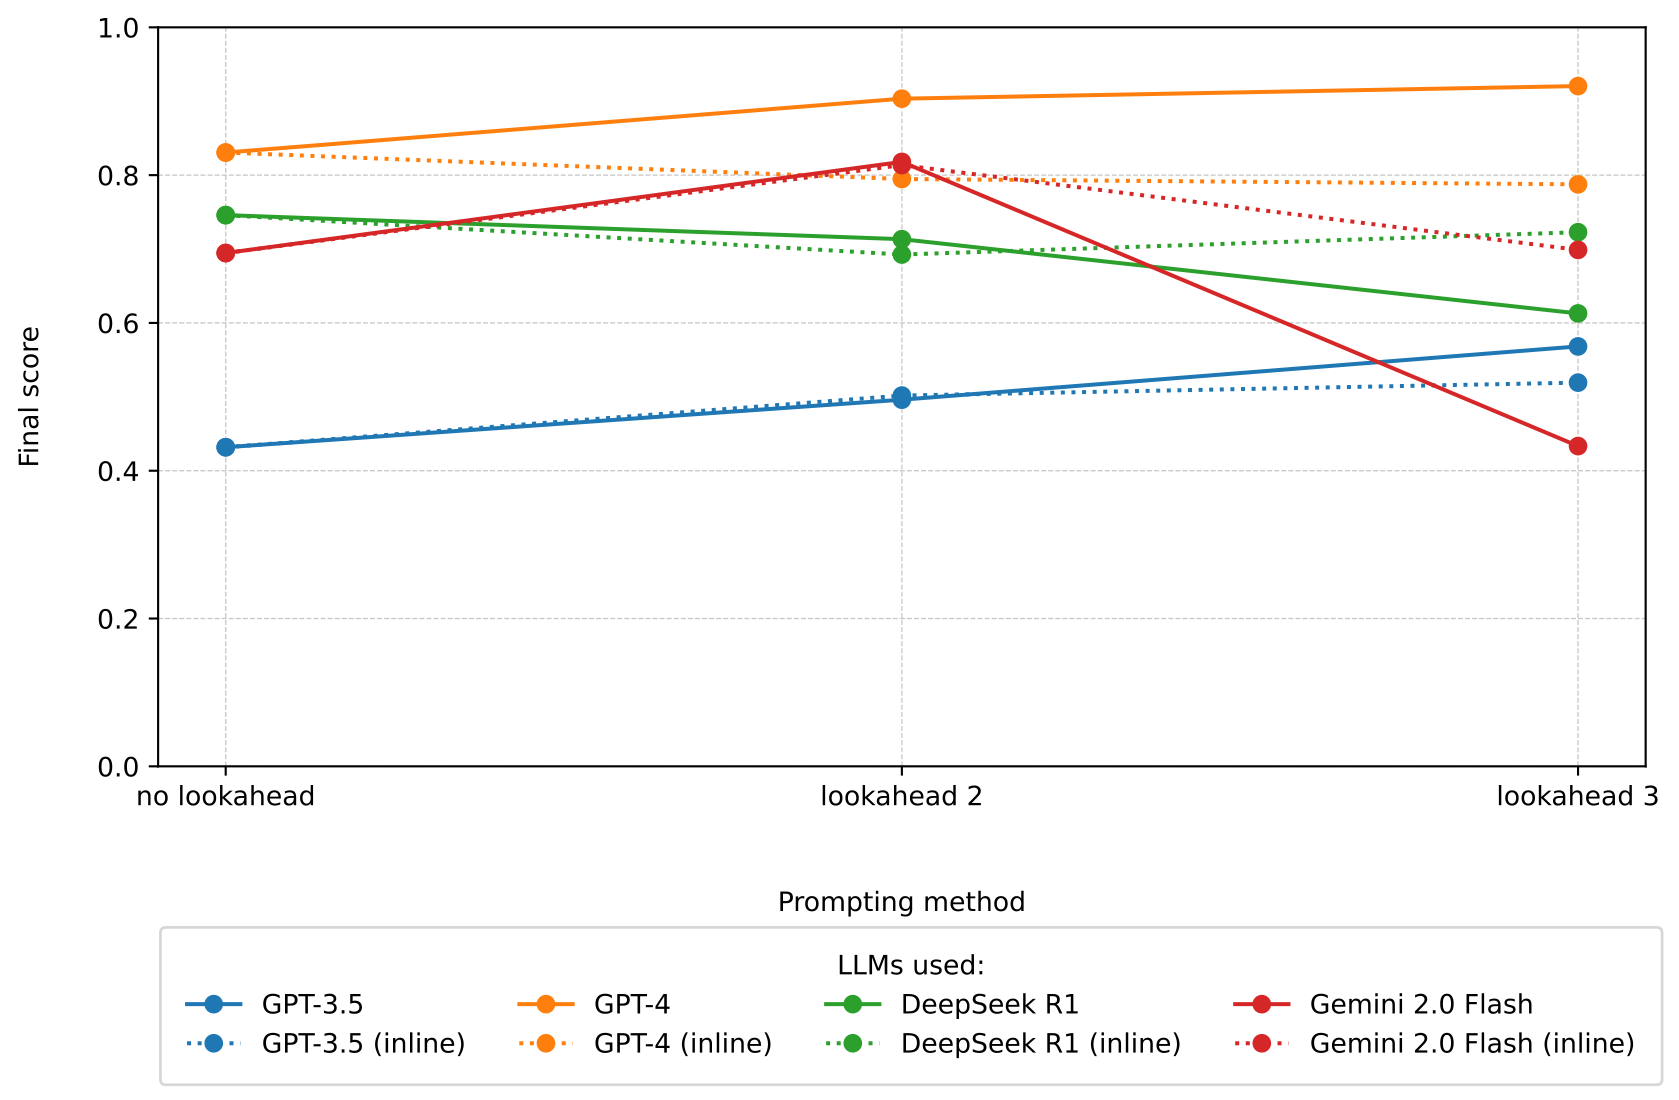
\includegraphics[width=0.7\textwidth]{fig/llm.png}
\caption{A plot showing the average scores for two different large language models (GPT-3.5 and GPT-4)
solving 20 challenge problems using five different prompting strategies.}
\label{fig:methods}
\end{figure}

The results suggest that, when using a more advanced LLM system, the ratio of correct
recommendations is high-enough to be practically useful. It also shows that providing more
information to the LLM through the lookahead mechanism improves the quality of the recommendation,
in a consistent way across multiple LLM systems. Arguably, offering a recommendation is preferrable
over providing an opaque solution, because it keeps the human in the loop \cite{sellen-2024-copilot}
and avoids ``ironies of automation'' \cite{bainbridge-1983-ironies} including deskilling.

\subparagraph{Generalised LLM assistant.}
The LLM-based recommendation engine developed for The Gamma can be implemented for any
choose-your-own-adventure system. As can be seen in Figure~\ref{fig:llm}, the information needed
to construct an LLM prompt comprise only the natural language query entered by the user,
a sequence of previously made choices $\iota_1, \ldots, \iota_{n-1}$ and the identifiers
$\iota_n, \iota_n', \iota_n'', \ldots$ of the choices offered by the $\choices$ operation.
As the LLM-based recommendations are based on natural language analysis of the prompt,
the quality of the recommendations depends on how semantically meaningful the generated
identifiers are.

An LLM-based recommendation engine can be useful for a number of the choose-your-own-adventure
interactive systems discussed in this paper:

\begin{itemize}
\setlength{\itemsep}{5pt}
\item We demonstrated the usefulness of the system for data exploration in The Gamma.
  Type providers for structured data \cite{petricek-2016-fsdata} typically generate small number
  of choices that the user can navigate without assistance, but navigating the schemas generated by
  type providers for semantic knowledge bases \cite{syme-2012-inforich} may be simplified through a
  natural language query.
\item The datadiff AI assistant discussed in Section~\ref{sec:motivation} matches columns based
  on statistical distribution and ignores column names. An LLM-based recommendation engine is
  useful in this case, because it is able to recommend the option \ident{Don't match
  `Urban.rural' and `Nation'} based solely on its name. For other AI assistants, the LLM-based
  recommendation engine would need access to the input data in order to be useful.
\item The problem of predicting steps in order to construct a proof is known as
  proofstep generation in literature focused on deep learning for theorem
  proving~\cite{zhaoyu-2024-deep}. Although most systems use models trained specifically for the
  task, there is also interest in using general-purpose LLMs~\cite{zhang-2023-proofs}.
  Our approach suggests a potential prompting strategy.
\end{itemize}

It is interesting to note that the choose-your-own-adventure calculus provides a common structure
that makes it possible to integrate multiple different approaches to assisting human in program
construction, ranging from automatic search (if we can provide a suitable heuristic) to
the use of LLMs (if generated choices carry enough semantic information). It can also serve as the
basis for visual programming environments discussed next.

\begin{figure}[t]
  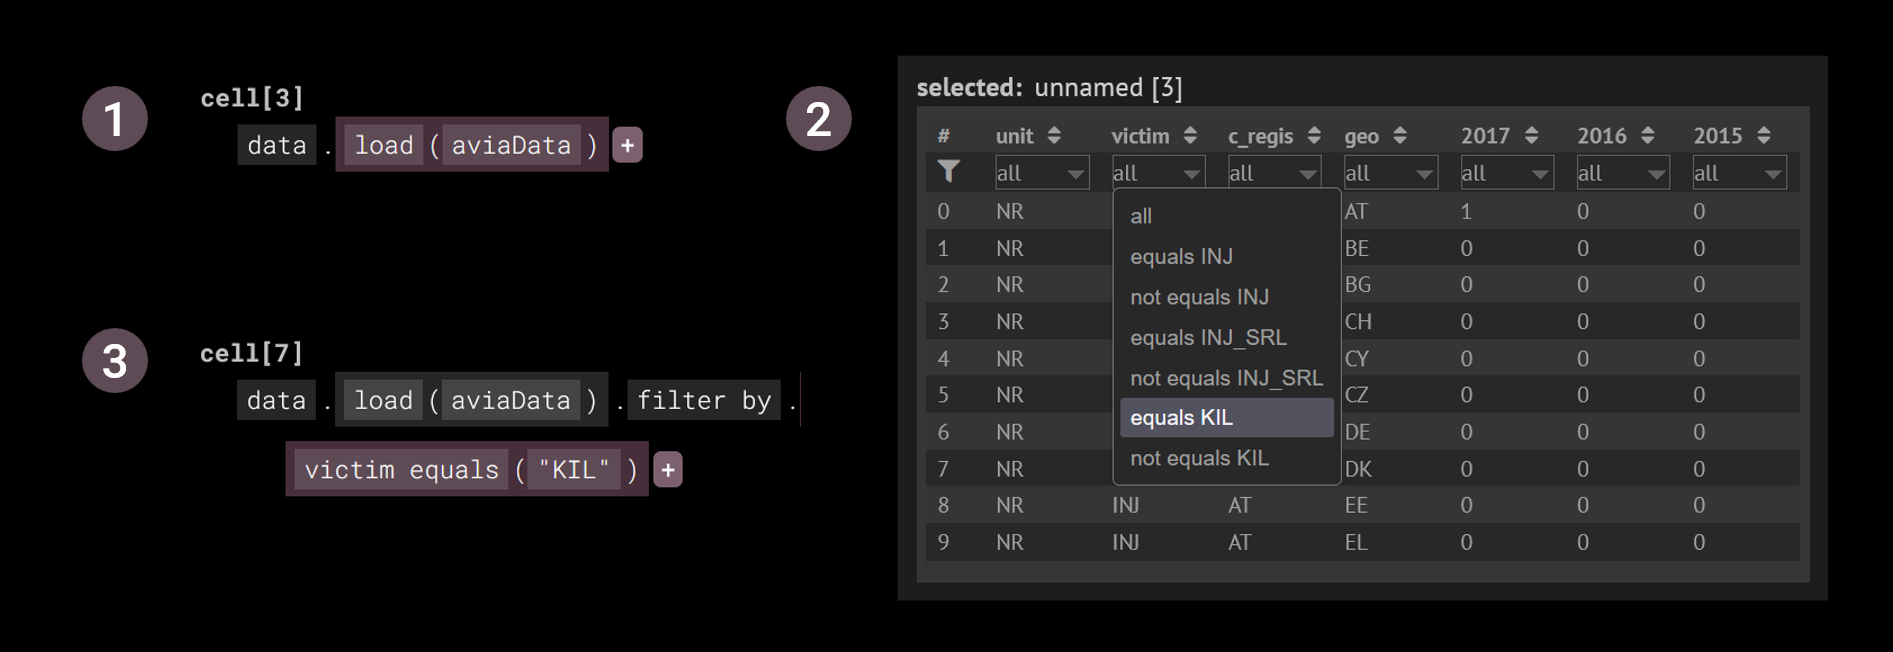
\includegraphics[width=0.9\textwidth]{fig/histogram.png}
  \caption{Programming by demonstration in Histogram -- (1) the user constructs program to load
    data, (2) then they filter data using graphical interface, which (3) records an operation
    corresponding to the interaction in code.}
  \label{fig:histogram}
\end{figure}

\subsection{Direct manipulation}

The Histogram programming environment~\cite{petricek-2019-histogram} provides a code completion
mechanism that can be used both to choose operations (as with type providers) and to specify
their parameters (by offering available values in context as possible arguments). It makes it
possible to evaluate sub-expressions at a fine-grained level and also refines type information
based on runtime values. However, it also supports programming by demonstration
\cite{cypher-1993-pbd,kandel-2011-wrangler}.

As illustrated in Figure~\ref{fig:histogram}, when the user loads data, they can manipulate it
in a table through a direct manipulation interface~\cite{shneiderman-1983-direct}. In Histogram,
interacting with the table triggers a sequence of operations that construct code. A similar
functionality is available in The Gamma, where operations for manipulating tabular data can be
selected not only through auto-completion, but also by interacting with the live preview.

The choose-your-own-adventure calculus enables a more general perspective on the programming
by demonstration interaction as implemented by Histogram. When interacting with a live
preview, the user is using a graphical interface to choose an option offered by $\choices$.
The operation appends an item to the sequence of choices, updates the system state
and generates a new preview where the choice is reflected (e.g., by filtering the table).

An interesting question is whether a program can be constructed solely through direct manipulation,
by interacting with the live previews. For this to be possible, the live preview needs to
offer links to all the possible options offered by $\choices$. This requires a careful design
of live previews. In Histogram (Figure~\ref{fig:histogram}), the live preview offers interactive
elements for filtering based on equality test (row of drop-downs), sorting (up/down arrows)
and indexing (indices in the ``\#'' column), but some operations (such as aggregation) can only
be constructed through code. Previews in The Gamma provide interactive elements for all options,
but those cannot always be integrated with the data display. For example, after choosing a grouping
key (Figure~\ref{fig:groupby}), the preview shows the key column, but other columns are hidden.
Specifying an aggregation thus requires an additional (somewhat arbitrary) ``+'' button that
provides access to the available choices.

\begin{figure}[t]
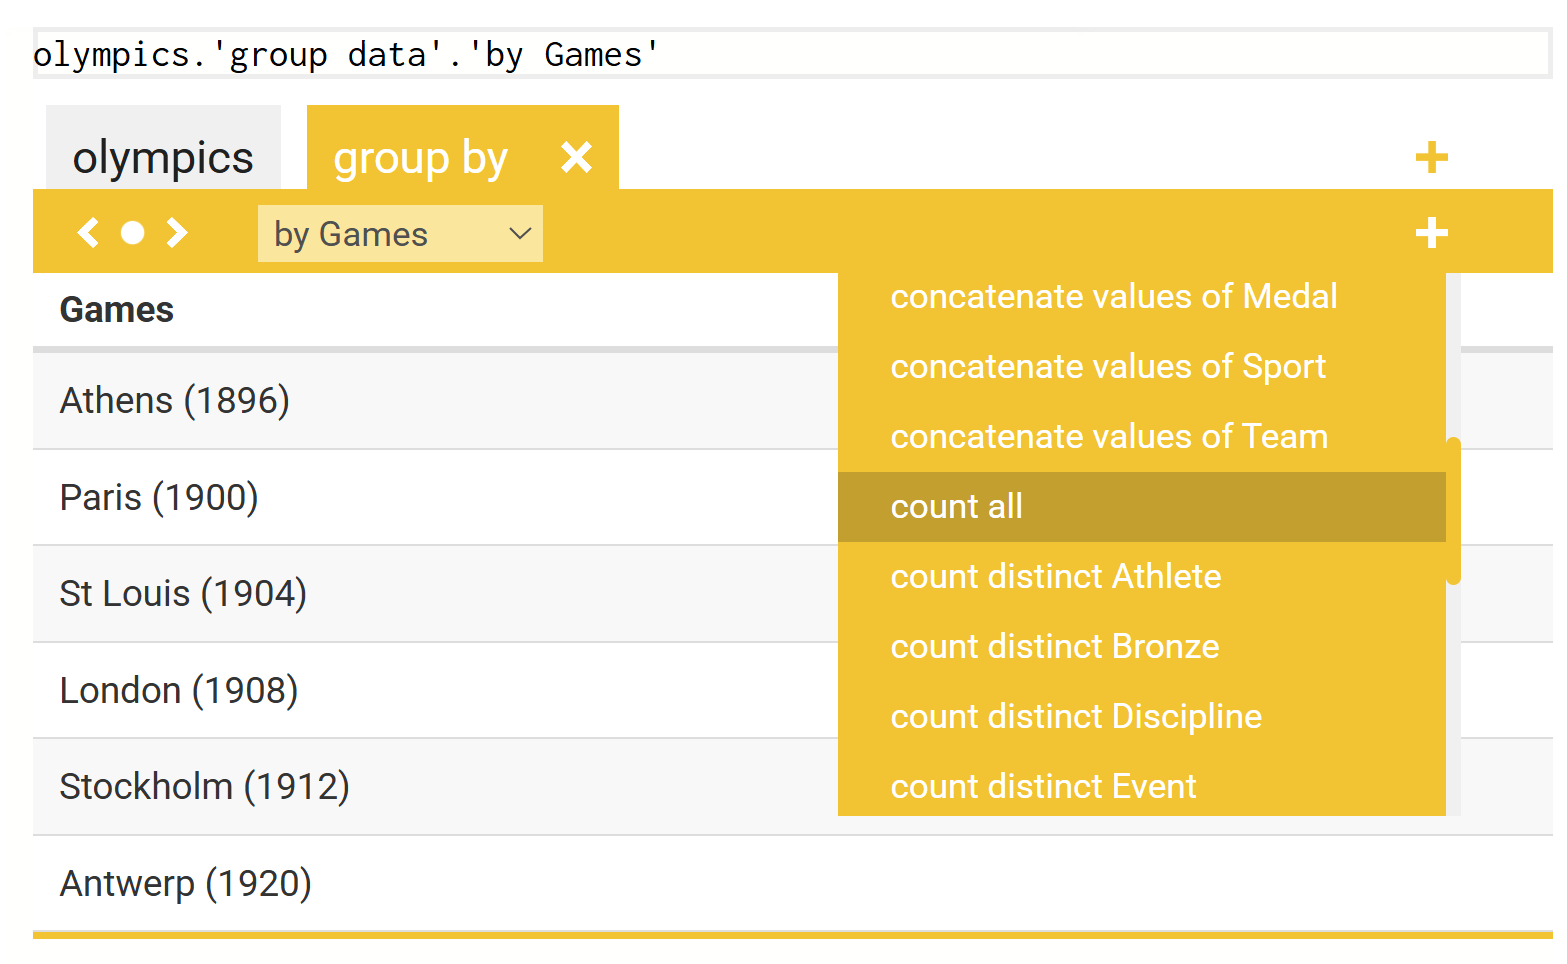
\includegraphics[width=0.6\textwidth]{fig/thegamma3.png}
\caption{Specifying aggregation in The Gamma through a live preview. Grouping keys can be
  selected from a drop-down, while aggregations have to be added through a menu.}
\label{fig:groupby}
\end{figure}

We can use the choose-your-own-adventure calculus to make the question whether all
programs can be constructed through direct manipulation more precise. Assume
$\preview(e)=p$ is a preview constructed for an expression $e$ and $\links(p)=\iota_1, \ldots, \iota_n$
are identifiers that can be invoked through the preview (akin to links in a hypertext document).

\begin{definition}[Direct manipulation]
A choose-your-own-adventure system with previews defined by $\preview$ and $\links$ supports
full direct manipulation if:
\begin{itemize}
\item $\forall \sigma, e$ such that $\select(\sigma)=e$ it is the case that
  $\forall \iota'\mapsto\sigma'\in\choices(\sigma)\,.\,\iota'\!\in\!\links(\preview(e))$.
\end{itemize}
\end{definition}

A system supports full direct manipulation if any program can be constructed by interacting with
the live previews, created based on the gradually constructed programs. As illustrated by The Gamma,
this can always be achieved by listing the options in a menu, but it is more interesting to see
if the links can be directly embedded in the preview as in the data table interface of Histogram.

The idea of directly mapping elements in a user interface to underlying structure of the
programming system has previously been implemented in pioneering user interface systems
including the Alternate Reality Kit~\cite{randall-1986-ark} and the Morphic framework for
Self and Squeak \cite{maloney-1995-morphic,maloney-2001-morphic}. In those systems, user interface
interactions directly map to messages sent to the underlying object and the halo element in
Morphic plays a similar role to the additional menu in The Gamma. It remains to be seen if
the choose-your-own-adventure calculus can provide a new way of looking at those systems.

\section{Limitations}
\label{sec:limitations}

TODO: Is this too general to be practically useful? E.g. LLM for interactive theorem provers
arguably needs more specific information.

\noindent
TODO: Something about unnecessary seqentialization

~

\noindent
TODO: What if the list of choices is infinite?

~

\noindent
TODO: How do you go back and revisit earlier choices? Backtracking in theorem provers or
fixing earlier part of the query in data exploration. Sometimes, you can retrace the
steps, but they may change...

~

\noindent
Related work - mbark for emacs, VS code command palette

~

\noindent
Alphageometry paper - follows a similar way of working to choose-your-own-adventure

\section{Conclusions}

TODO: Some conclusions
1) lets us ask all those questions
2) let ideas cross between domains

\newpage


\bibliography{paper}


































\end{document}
